\documentclass[compress]{beamer}
\usepackage{ifthen,verbatim}

\title{Effect of Alignment Systematics on High Di-Muon Mass \\ (This analysis is still rather rough)}
\author{Jim Pivarski, Alexei Safonov}
\institute{Texas A\&M University}
\date{ 1 October, 2007}

\newcommand{\isnote}{}
\xdefinecolor{lightyellow}{rgb}{1.,1.,0.25}
\xdefinecolor{darkblue}{rgb}{0.1,0.1,0.7}
\xdefinecolor{pink}{rgb}{0.7,0.5,0.5}

%% Uncomment this to get annotations
%% \def\notes{\addtocounter{page}{-1}
%%            \renewcommand{\isnote}{*}
%% 	   \beamertemplateshadingbackground{lightyellow}{white}
%%            \begin{frame}
%%            \frametitle{Notes for the previous page (page \insertpagenumber)}
%%            \itemize}
%% \def\endnotes{\enditemize
%% 	      \end{frame}
%%               \beamertemplateshadingbackground{white}{white}
%%               \renewcommand{\isnote}{}}

%% Uncomment this to not get annotations
\def\notes{\comment}
\def\endnotes{\endcomment}

\setbeamertemplate{navigation symbols}{}
\setbeamertemplate{headline}{\includegraphics[height=1 cm]{../cmslogo} \hspace{0.1 cm} \includegraphics[height=1 cm]{../tamulogo} \hfill
\begin{minipage}{5.5 cm}
\vspace{-0.75 cm} \small
\begin{center}
\ifthenelse{\equal{\insertpagenumber}{1}}{}{\textcolor{blue}{\insertsection}}
\end{center}
\end{minipage} \hfill
\begin{minipage}{4.5 cm}
\vspace{-0.75 cm} \small
\begin{flushright}
\ifthenelse{\equal{\insertpagenumber}{1}}{}{Jim Pivarski \hspace{0.5 cm} \insertpagenumber\isnote/\pageref{numpages}}
\end{flushright}
\end{minipage}\mbox{\hspace{0.2 cm}}}

\begin{document}
\frame{\titlepage}

\begin{notes}
\item This is the annotated version of my talk.
\item If you want the version that I am presenting, download the one
labeled ``slides'' on Indico (or just ignore these yellow pages).
\item The annotated version is provided for extra detail and a written
record of comments that I intend to make orally.
\item Yellow notes refer to the content on the {\it previous} page.
\item All other slides are identical for the two versions.
\end{notes}

\begin{frame}
\frametitle{Figure of merit for a good alignment}

\begin{itemize}
\item I have been using accuracy as a figure of merit: RMS and core
fit of residual misalignment after an alignment process
\item But there is a different accuracy for each degree of freedom
\item and distributions can sometimes be non-Gaussian

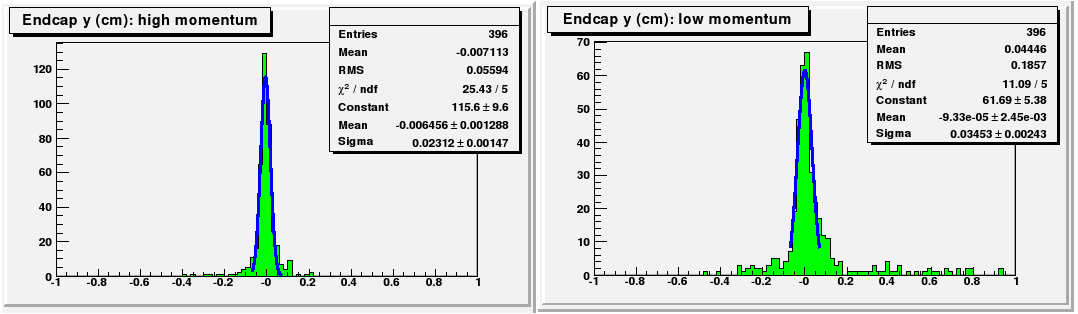
\includegraphics[width=\linewidth]{momentum_accuracy.png}

\item How important are e.g.\ $\phi_x$ and $y$ relative to $x$?

\item How important are tail contributions relative to core width?

\item $\Rightarrow$ look at consequences for physics
\end{itemize}
\end{frame}

\begin{frame}
\frametitle{Dependence on integrated luminosity: $Z$, $Z'$ resolution}
\vspace{0.25 cm}
\begin{columns}
\column{0.5\linewidth}
\begin{center}
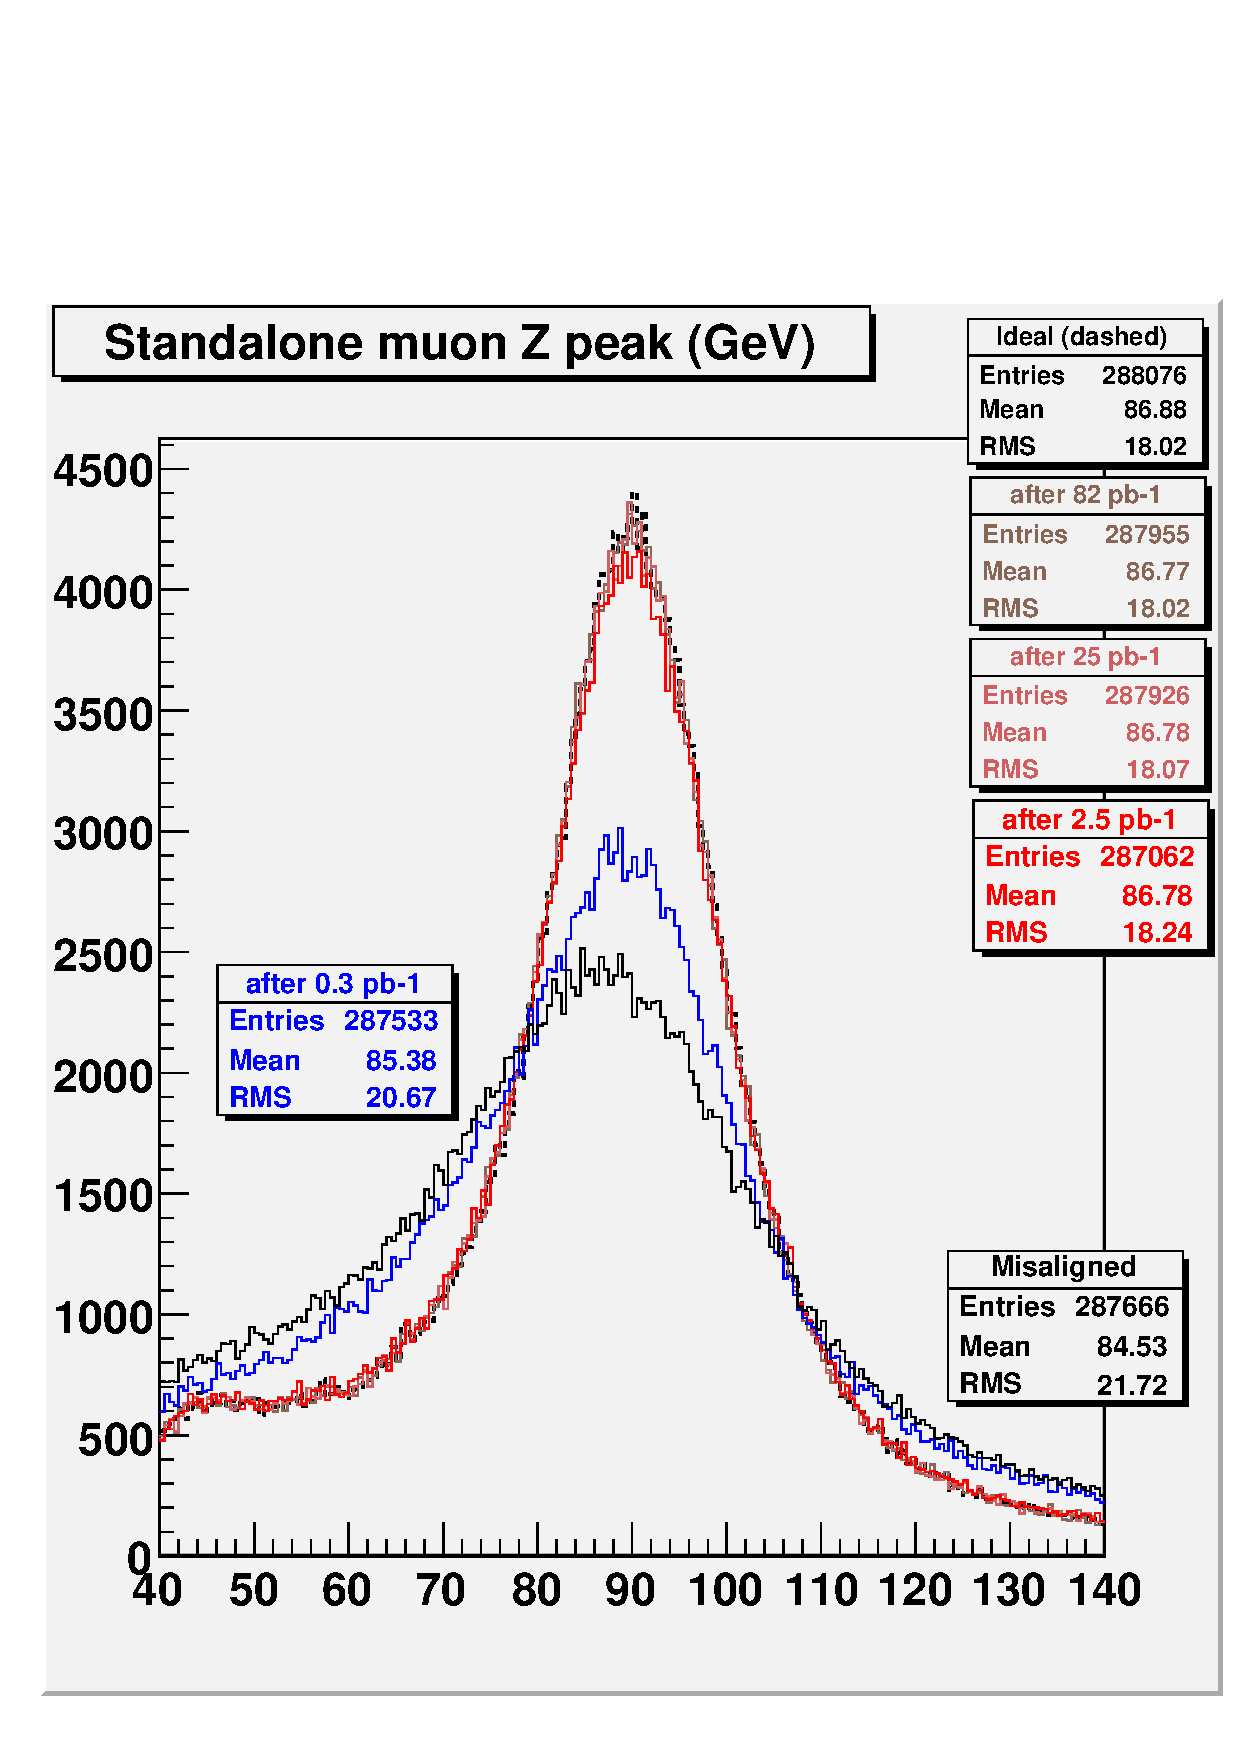
\includegraphics[width=0.9\linewidth]{checkit_standaloneZ.pdf}
\end{center}
\column{0.5\linewidth}
\begin{center}
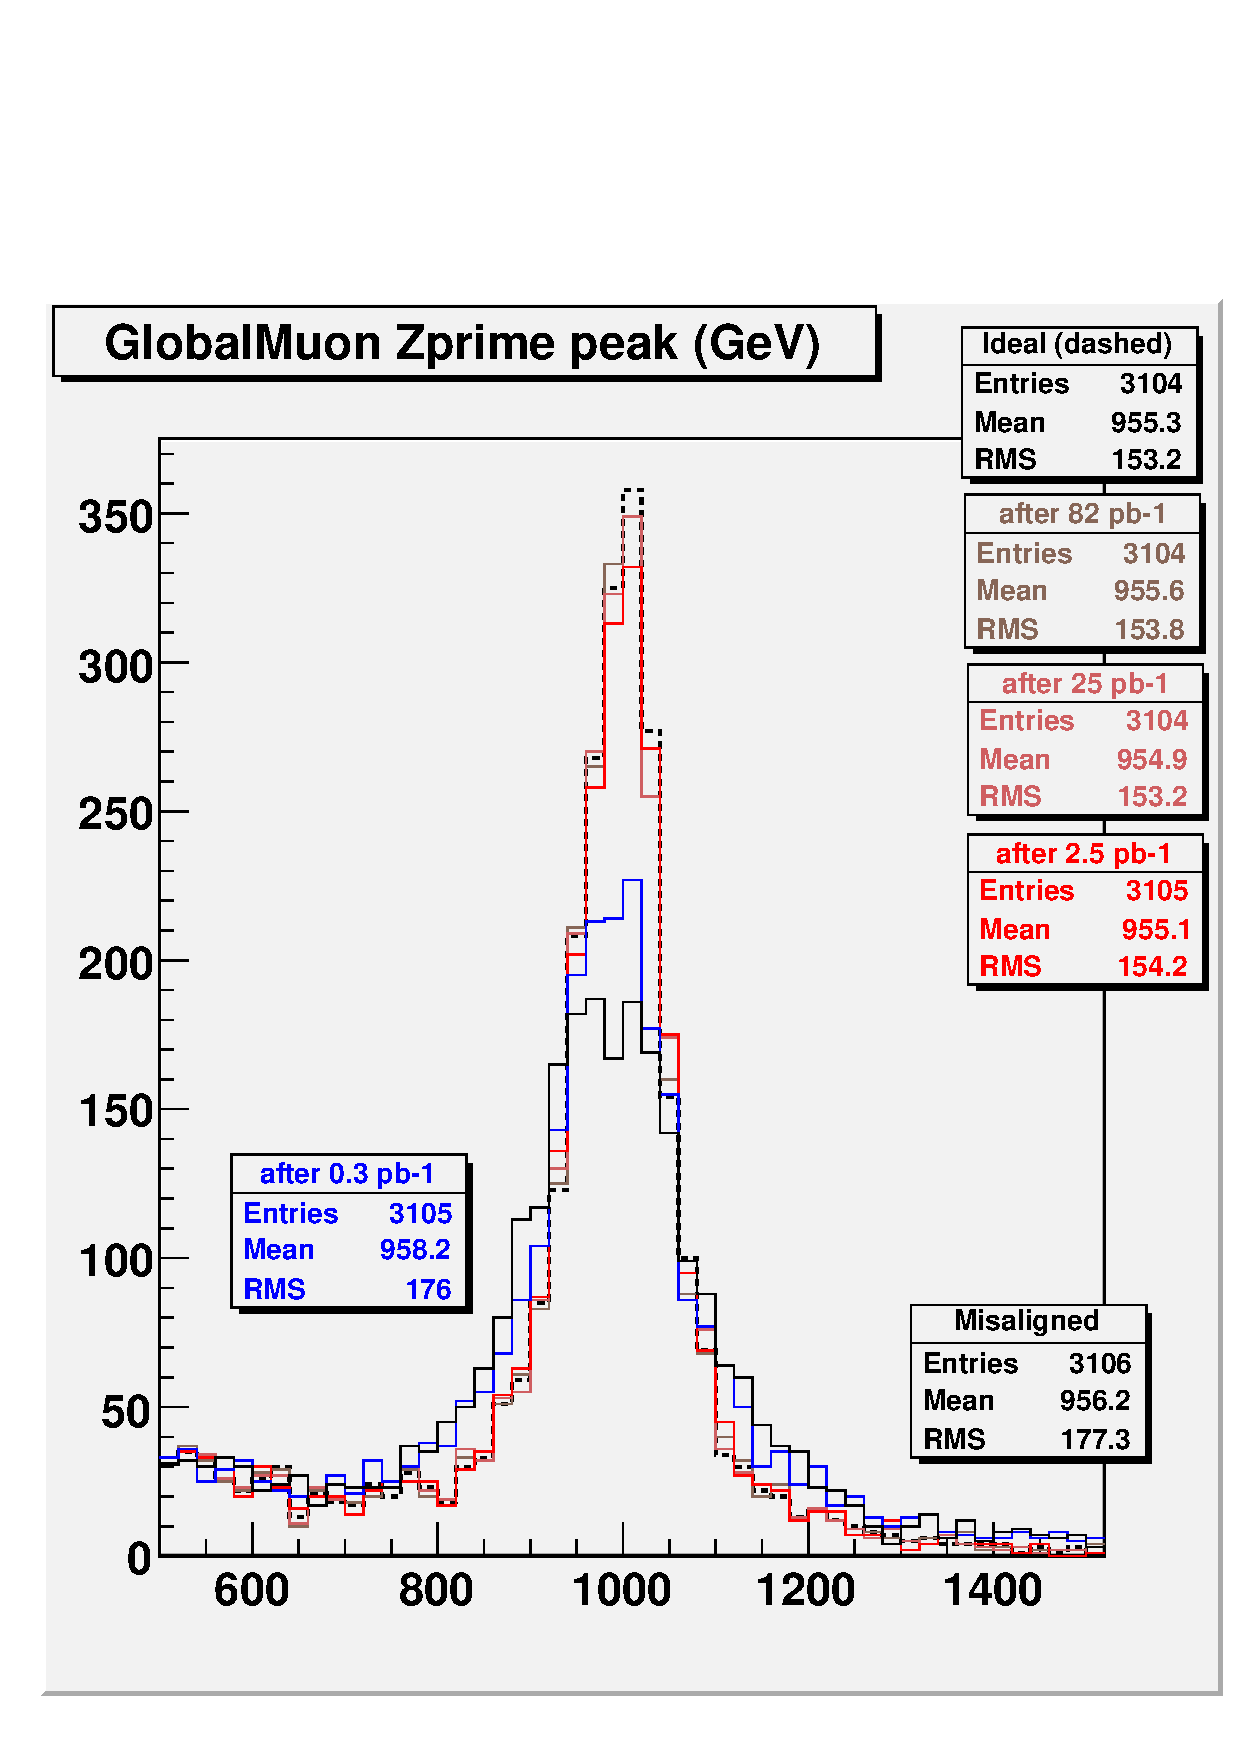
\includegraphics[width=0.9\linewidth]{checkit_globZprime.pdf}
\end{center}
\end{columns}

\vspace{0.25 cm}
\begin{itemize}
\item Muon alignment only influences $\sim$100~GeV muons in standalone mode; I'll focus on $\sim$1000~GeV
\end{itemize}
\vspace{-0.25 cm}
\mbox{ }

\end{frame}

\begin{frame}
\frametitle{Drell-Yan and $Z'$ at \only<1>{1}\only<2>{2} TeV}
\begin{columns}
\column{0.35\linewidth}
\only<1>{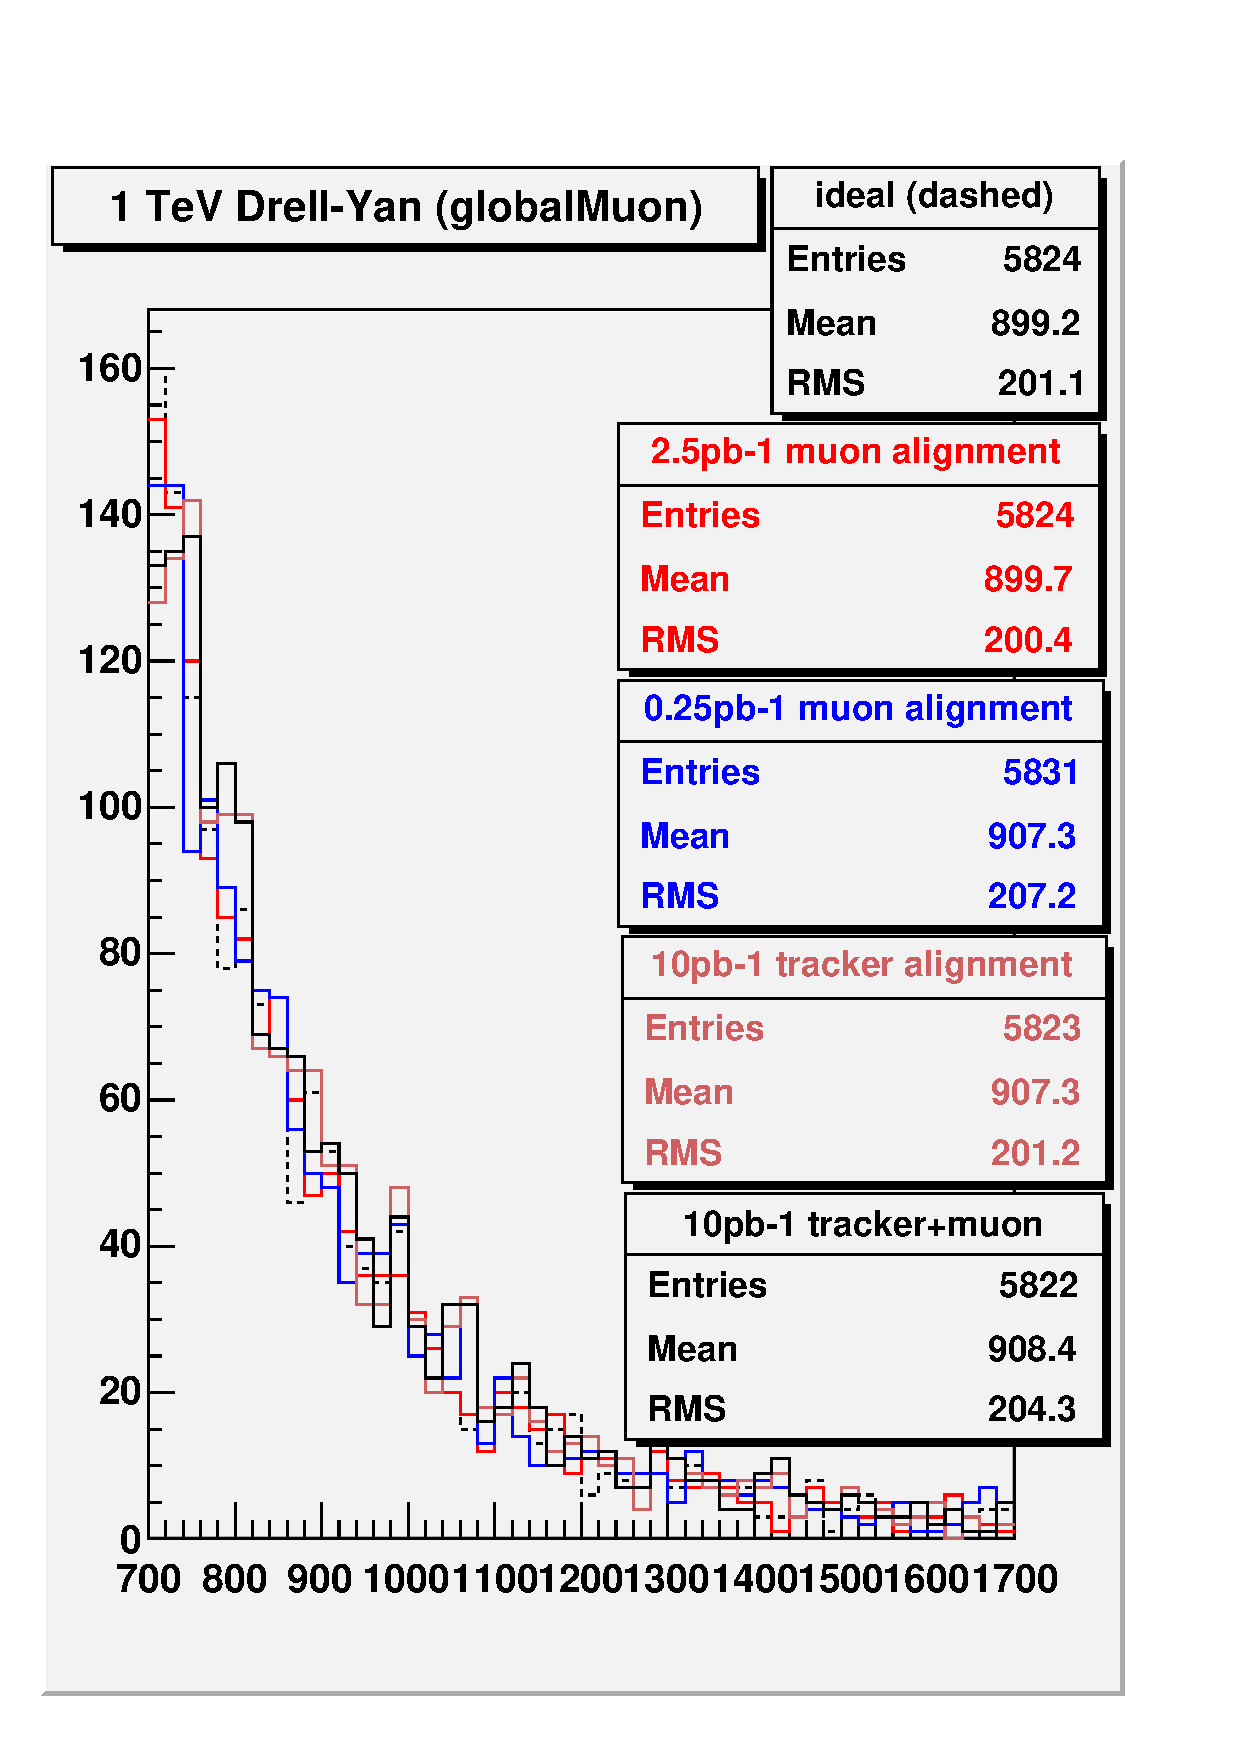
\includegraphics[width=\linewidth]{compare_dy_500.pdf}}
\only<2>{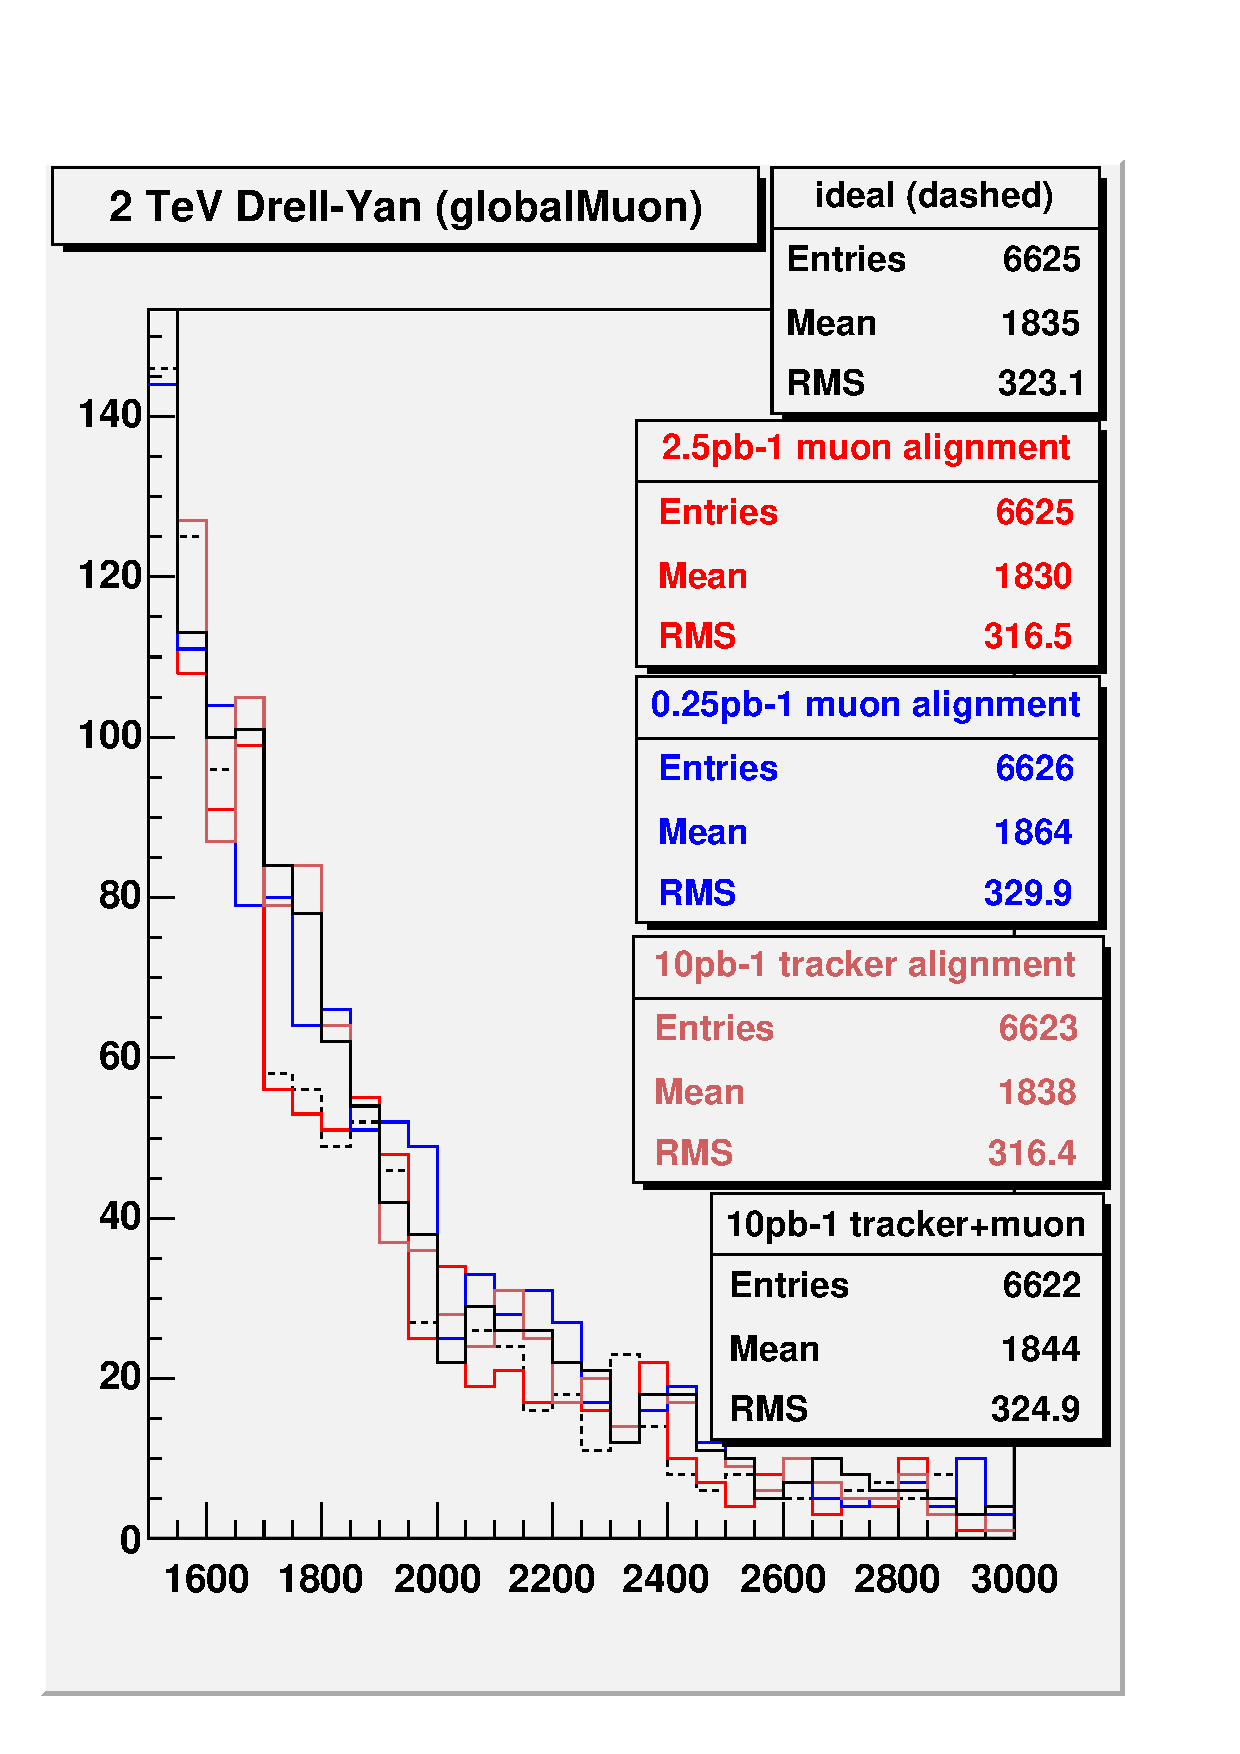
\includegraphics[width=\linewidth]{compare_dy_1000.pdf}}
\column{0.35\linewidth}
\only<1>{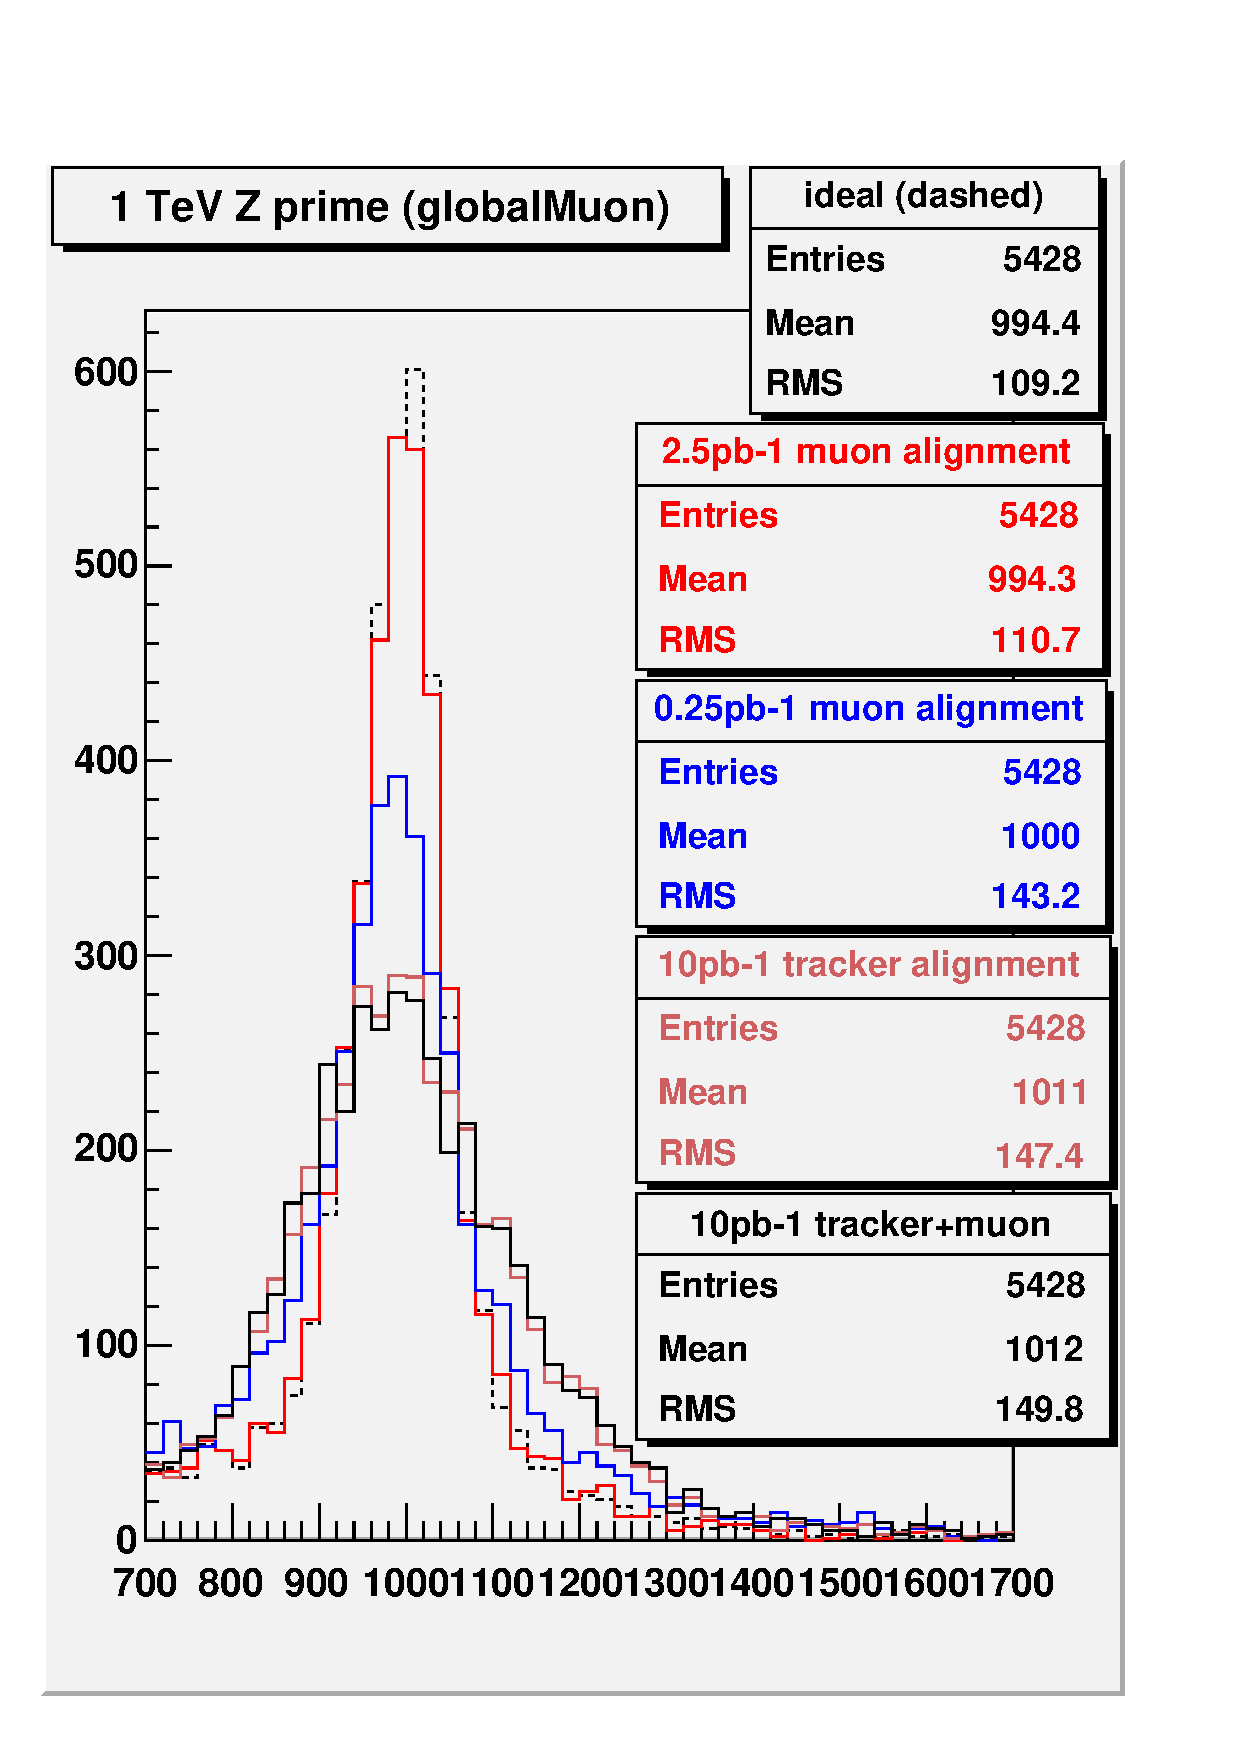
\includegraphics[width=\linewidth]{compare_zprime_1000.pdf}}
\only<2>{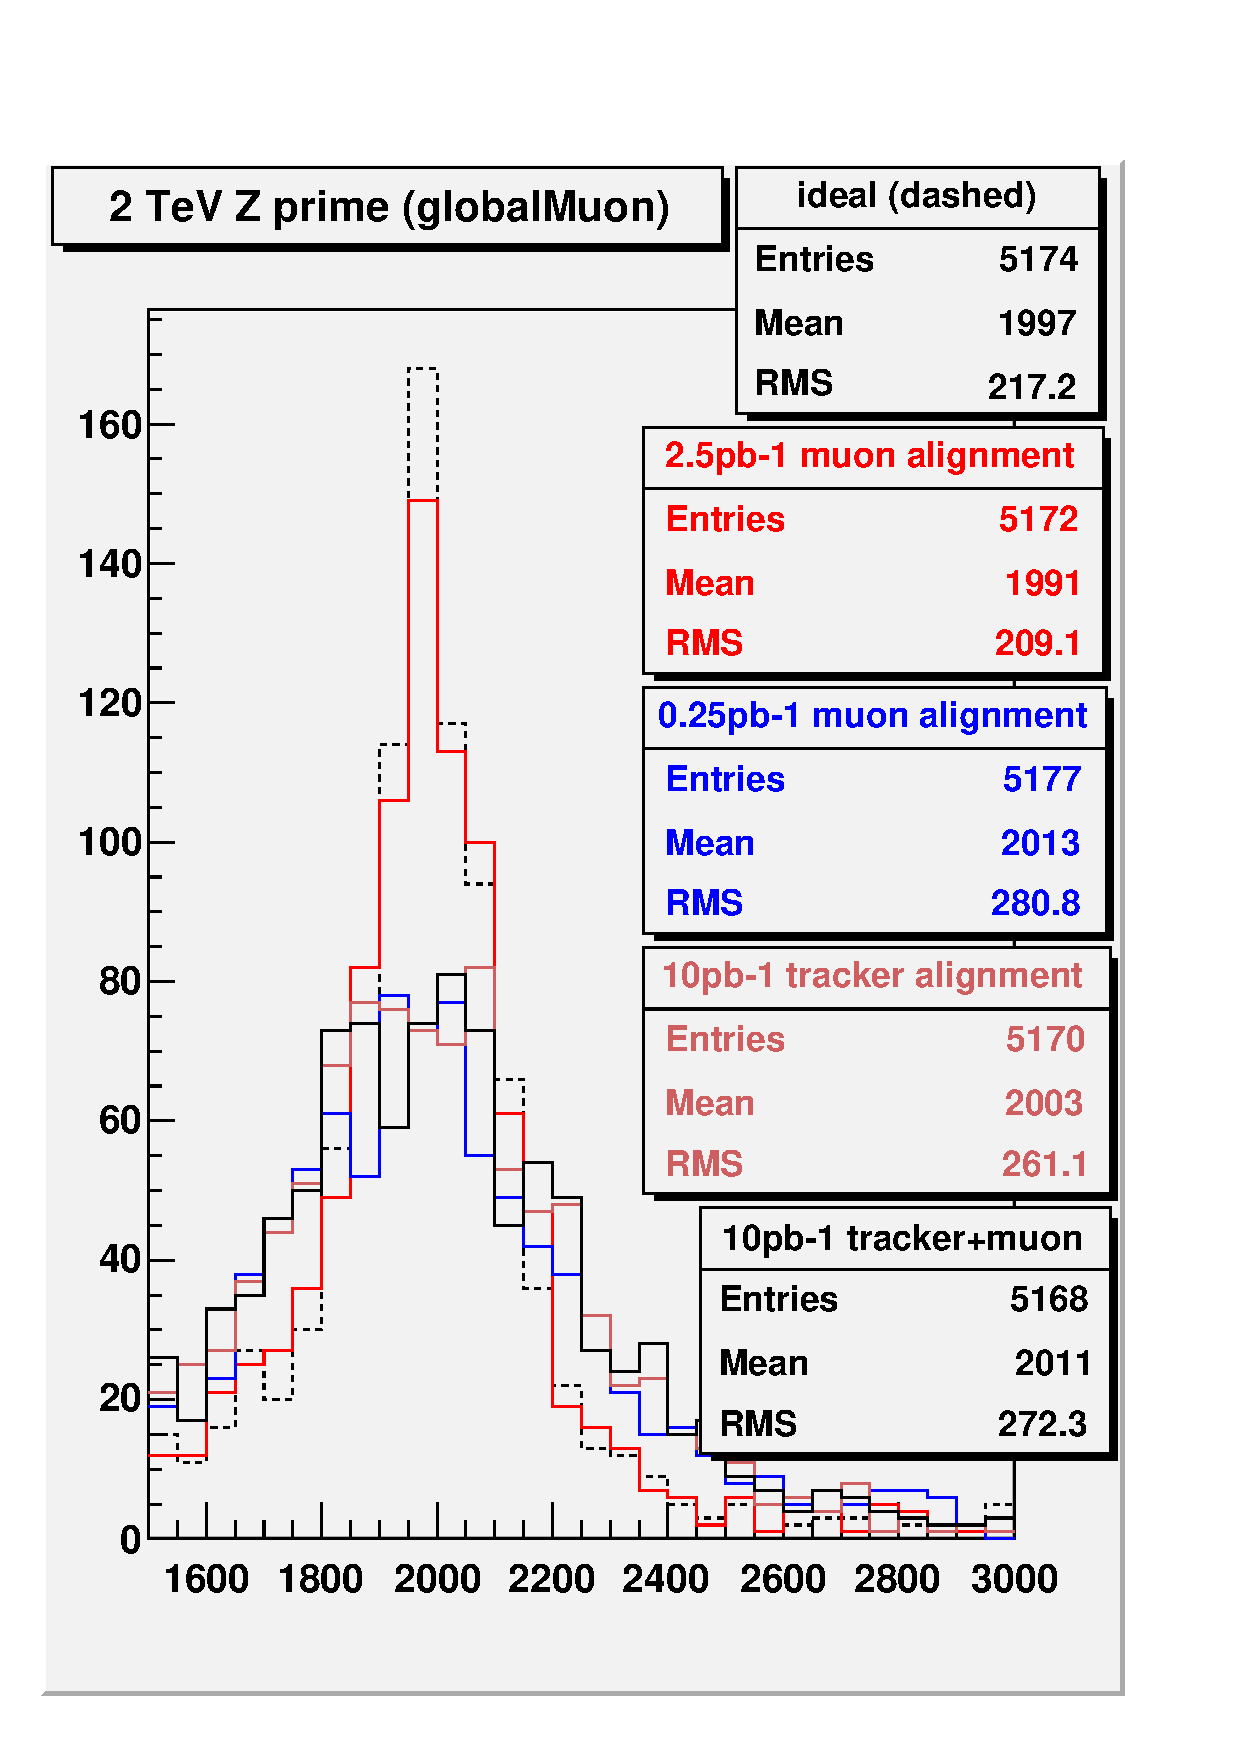
\includegraphics[width=\linewidth]{compare_zprime_2000.pdf}}
\column{0.3\linewidth}
\textcolor{red}{2.5~pb$^{-1}$ and} \textcolor{blue}{25~pb$^{-1}$ muon alignments} have ideal tracker

\vspace{0.3cm}
\textcolor{pink}{10~pb$^{-1}$ tracker alignment} is the standard scenario with ideal muon alignment
\end{columns}

\vspace{0.3cm}
tracker $+$ muon has both misaligned: muon alignment has small systematic errors from tracker $\to$ muon track extrapolation
\end{frame}

\begin{frame}
\frametitle{What's surprising to me: not much Drell-Yan smearing}
\begin{itemize}\setlength{\itemsep}{0.25 cm}
\item<1-> Drell-Yan is exponentially distributed: $f(x) = e^{-kx}$
\item<1-> Convoluted: $\displaystyle f(y) = \int f(x) \, \frac{1}{\sqrt{2\pi}\sigma} \exp\left(\frac{-(x-y)^2}{2\sigma^2}\right) \, dx$
\item<1-> $f(y) = e^{-ky} \, \exp(\sigma^2 k^2 / 2)$
\item<1-> Convolution kernel is a series: $A_1 e^{x^2/2/{\sigma_1}^2} + A_2 e^{x^2/2/{\sigma_2}^2} + \ldots$ (``tails'' are wide Gaussians with small contribution)
\item<1-> $f(y) = e^{-ky} (A_1 \exp({\sigma_1}^2 k^2 / 2) + A_2 \exp({\sigma_2}^2 k^2 / 2) + \ldots)$
\item<1-> Depends linearly on $A_i$ and as $e^{{\sigma_i}^2}$ on width: could be big!
\end{itemize}

\vfill
\begin{itemize}
\item<2->Fit Drell-Yan distributions: \hfill $k$ = 6$\times$10$^{-3}$/GeV (near 1 TeV) \\ \mbox{ } \hfill and 3.4$\times$10$^{-3}$/GeV (near 2 TeV)
\item<2->What's $\sigma$?
\end{itemize}
\end{frame}

\begin{frame}
\frametitle{Worst case: tracker $+$ muon misalignment}
\begin{columns}
\column{0.5\linewidth}
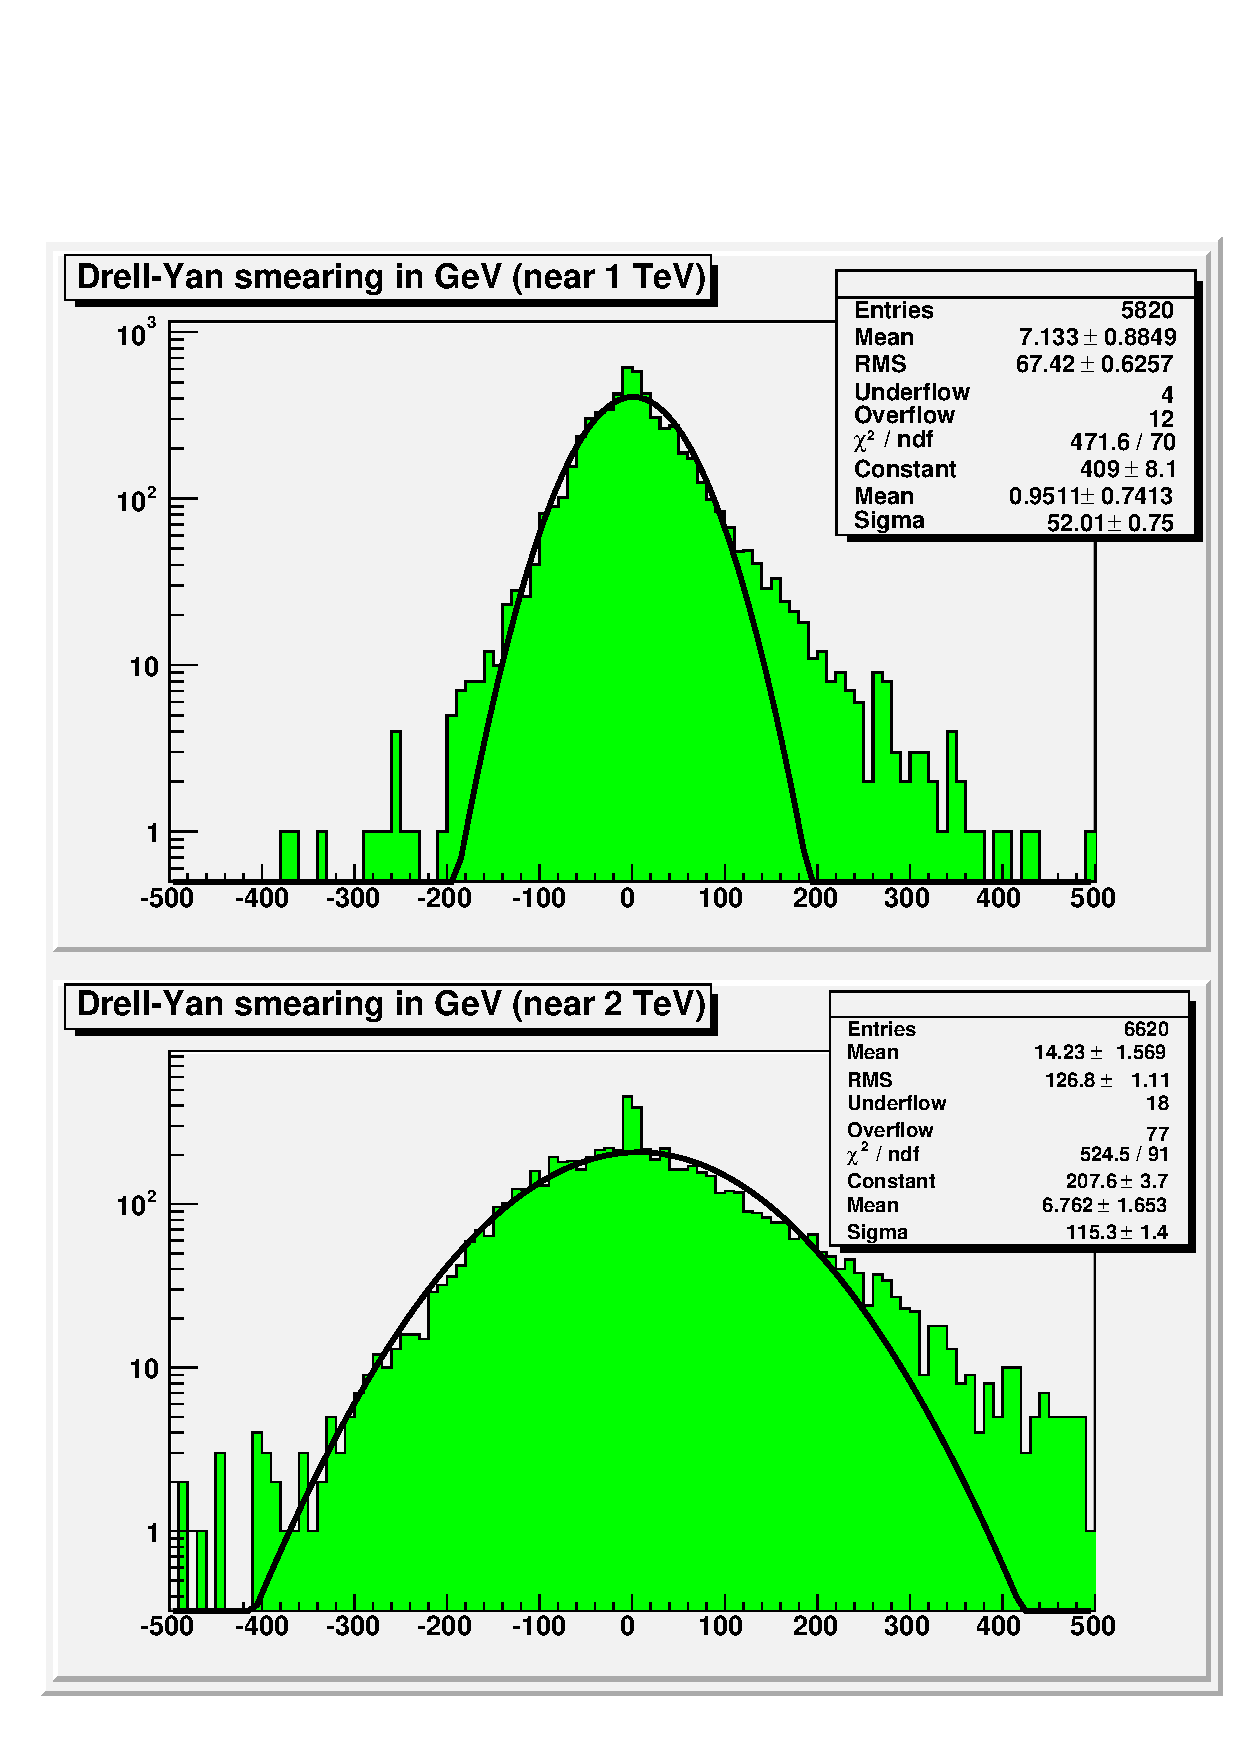
\includegraphics[width=\linewidth]{dy_smearing_inGeV.pdf}
\column{0.5\linewidth}
\begin{tabular}{c c c}
Sample & Central $\sigma$ & $e^{\sigma^2 k^2 / 2}$ \\\hline
Near 1~TeV & 52~GeV & 1.05 \\
Near 2~TeV & 115~GeV & 1.08 \\
\end{tabular}

\vspace{0.5 cm}
A Gaussian twice as wide would be down by a factor of $\sim$10:

\vspace{0.5 cm}
\begin{tabular}{c c c}
Sample & Tail $\sigma$ & $e^{\sigma^2 k^2 / 2}$ \\\hline
Near 1~TeV & 100~GeV & 1.21 \\
Near 2~TeV & 230~GeV & 1.36 \\
\end{tabular}

\vspace{0.5 cm}
0.9 $\times$ 1.08 $+$ 0.1 $\times$ 1.36 = 1.11

\end{columns}
\end{frame}

\begin{frame}
\frametitle{Worse than worst case: 2$\times$ tracker $+$ muon misalignment}
\begin{columns}
\column{0.5\linewidth}
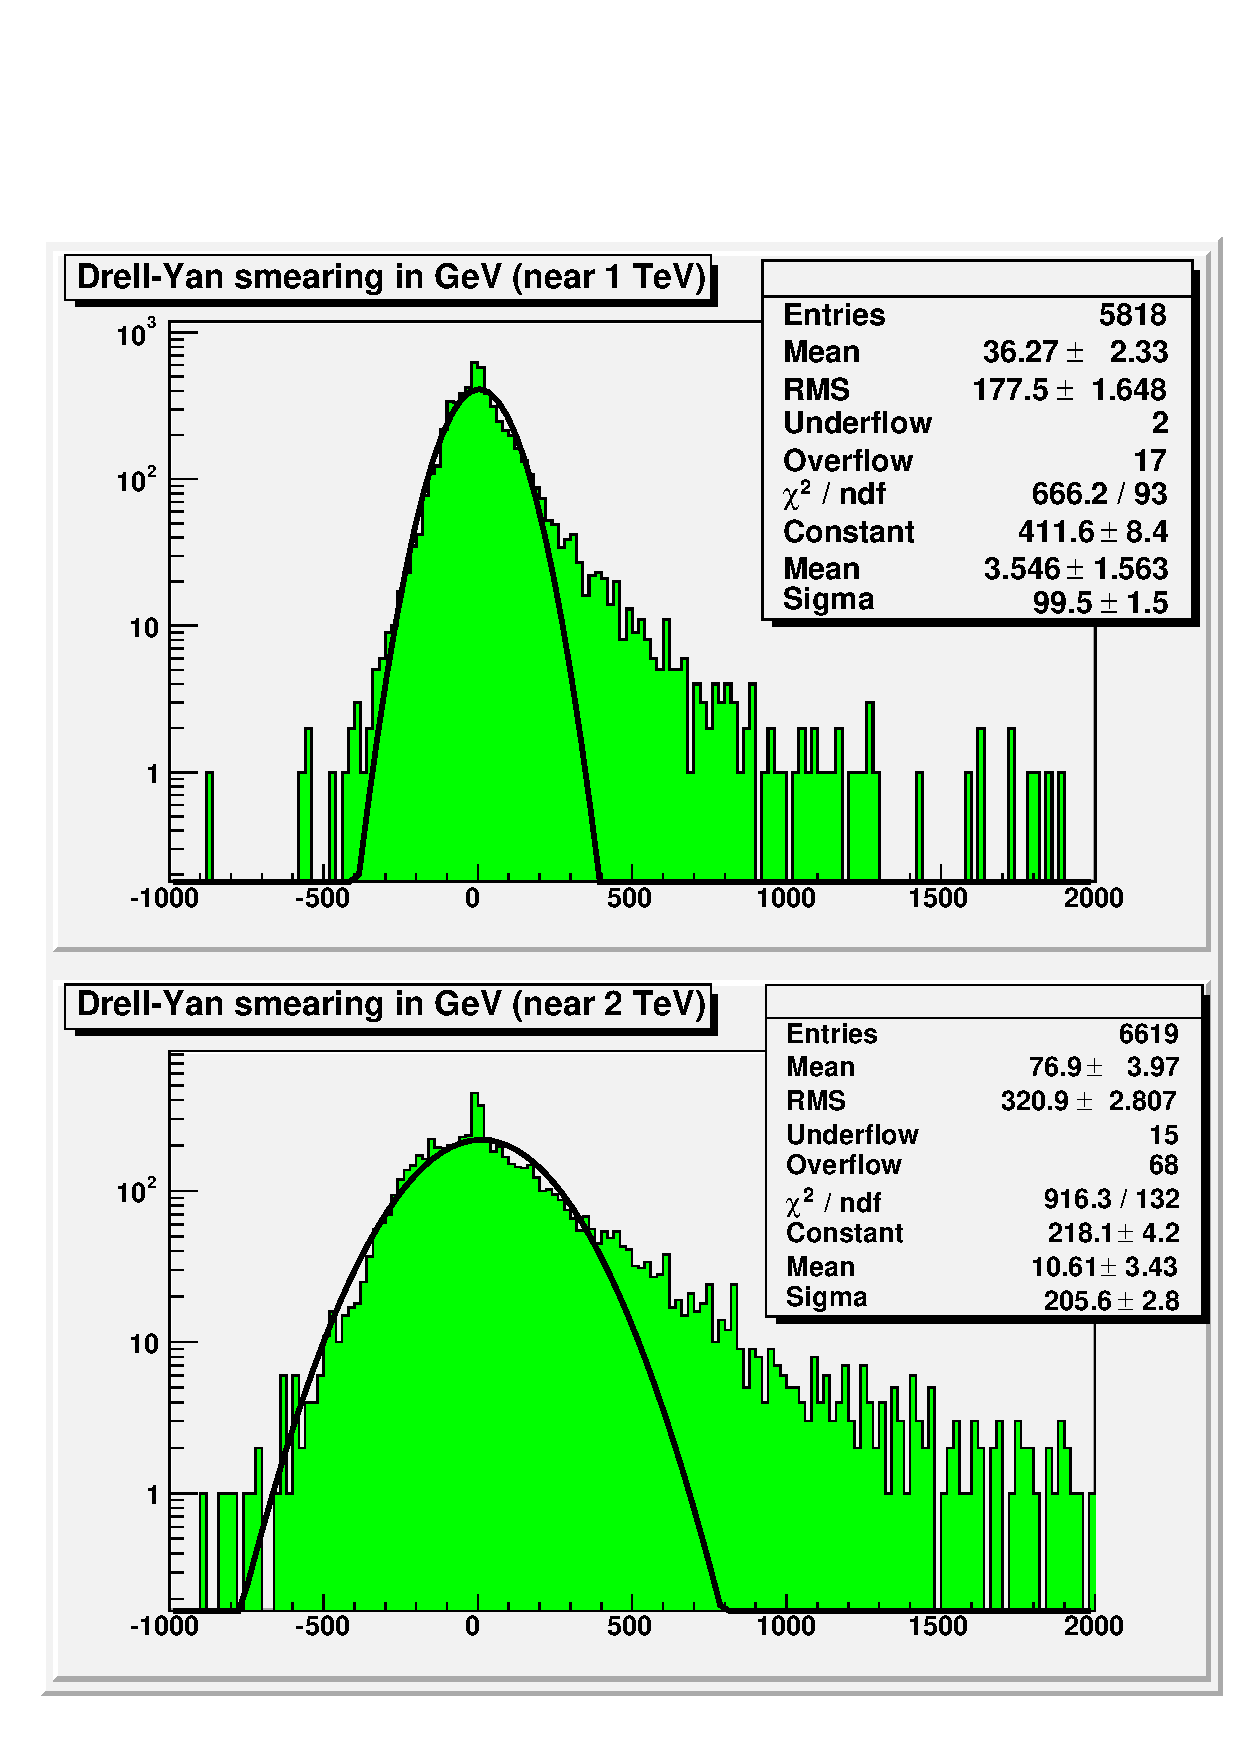
\includegraphics[width=\linewidth]{dy_smearing_inGeV_tracker2.pdf}
\column{0.5\linewidth}
Estimates of Gaussian series

\vspace{0.1 cm}
\begin{tabular}{c c c}
$A_i$ & Width & $A_i \, e^{{\sigma_i}^2 k^2 / 2}$ \\\hline
0.9 & 100~GeV & 1.08 \\
0.1 & 200~GeV & 0.21 \\
0.01 & 300~GeV & 0.05 \\\hline
& & 1.34 \\
\end{tabular}

\vspace{0.5 cm}
Estimates of Gaussian series

\vspace{0.1 cm}
\begin{tabular}{c c c}
$A_i$ & Width & $A_i \, e^{{\sigma_i}^2 k^2 / 2}$ \\\hline
0.9 & 205~GeV & 1.15 \\
0.1 & 300~GeV & 0.07 \\
0.01 & 400~GeV & 0.03 \\\hline
& & 1.25 \\
\end{tabular}

\end{columns}
\end{frame}

\begin{frame}
\frametitle{Conclusions for Drell-Yan smearing}

\begin{itemize}\setlength{\itemsep}{0.5 cm}
\item Not as bad as I imagined: smallness of $k$ wins over $\sigma$

\item I need a better way to fit double-, triple-, or $N$le-Gaussians

\item or maybe an expansion series, like Taylor or Fourier (I couldn't find one)

\item There must be a threshold where $A_i \, e^{{\sigma_i}^2 k^2 /
2}$ explodes: how close are we to that threshold?
\end{itemize}
\end{frame}

\begin{frame}
\frametitle{Event-by-event effect of alignment}
\begin{columns}
\column{0.5\linewidth}
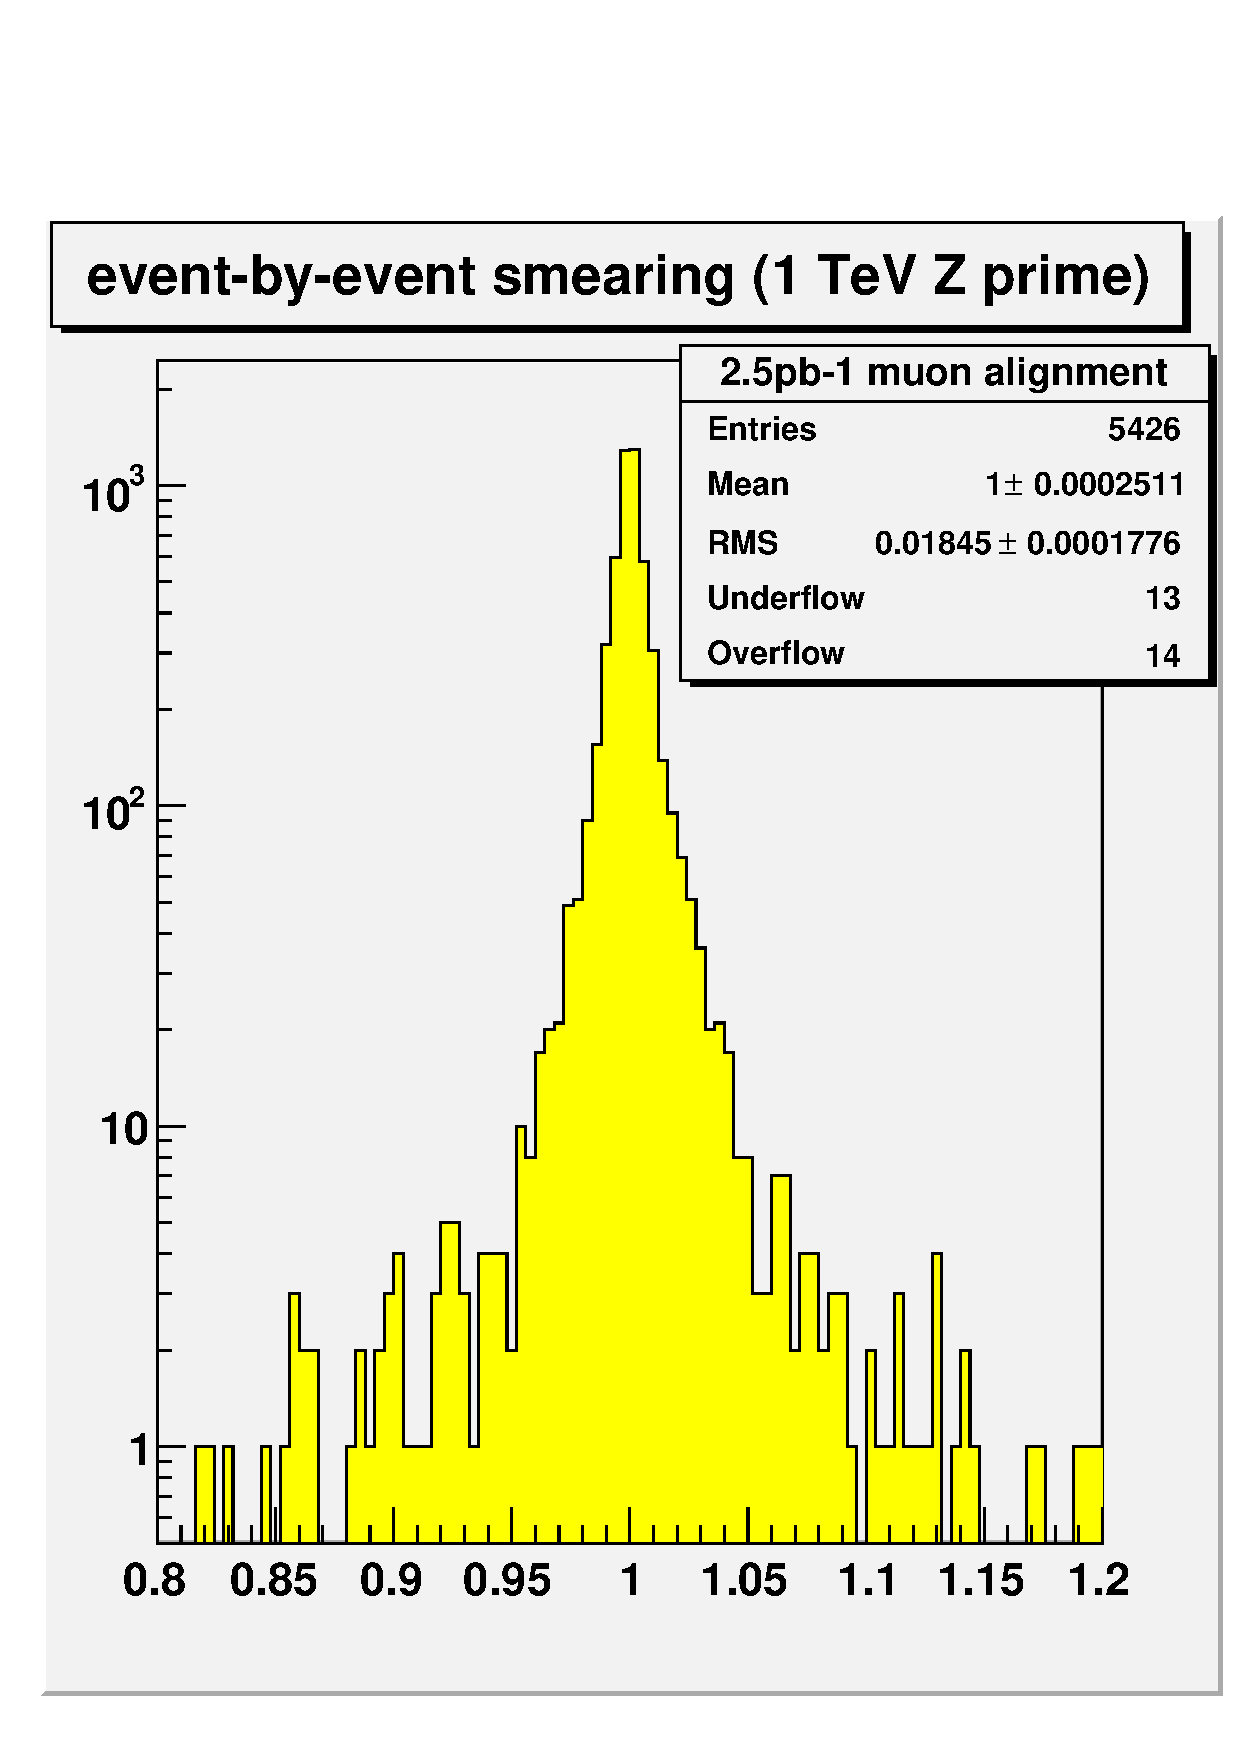
\includegraphics[width=\linewidth]{smearing_events10k.pdf}
\column{0.5\linewidth}
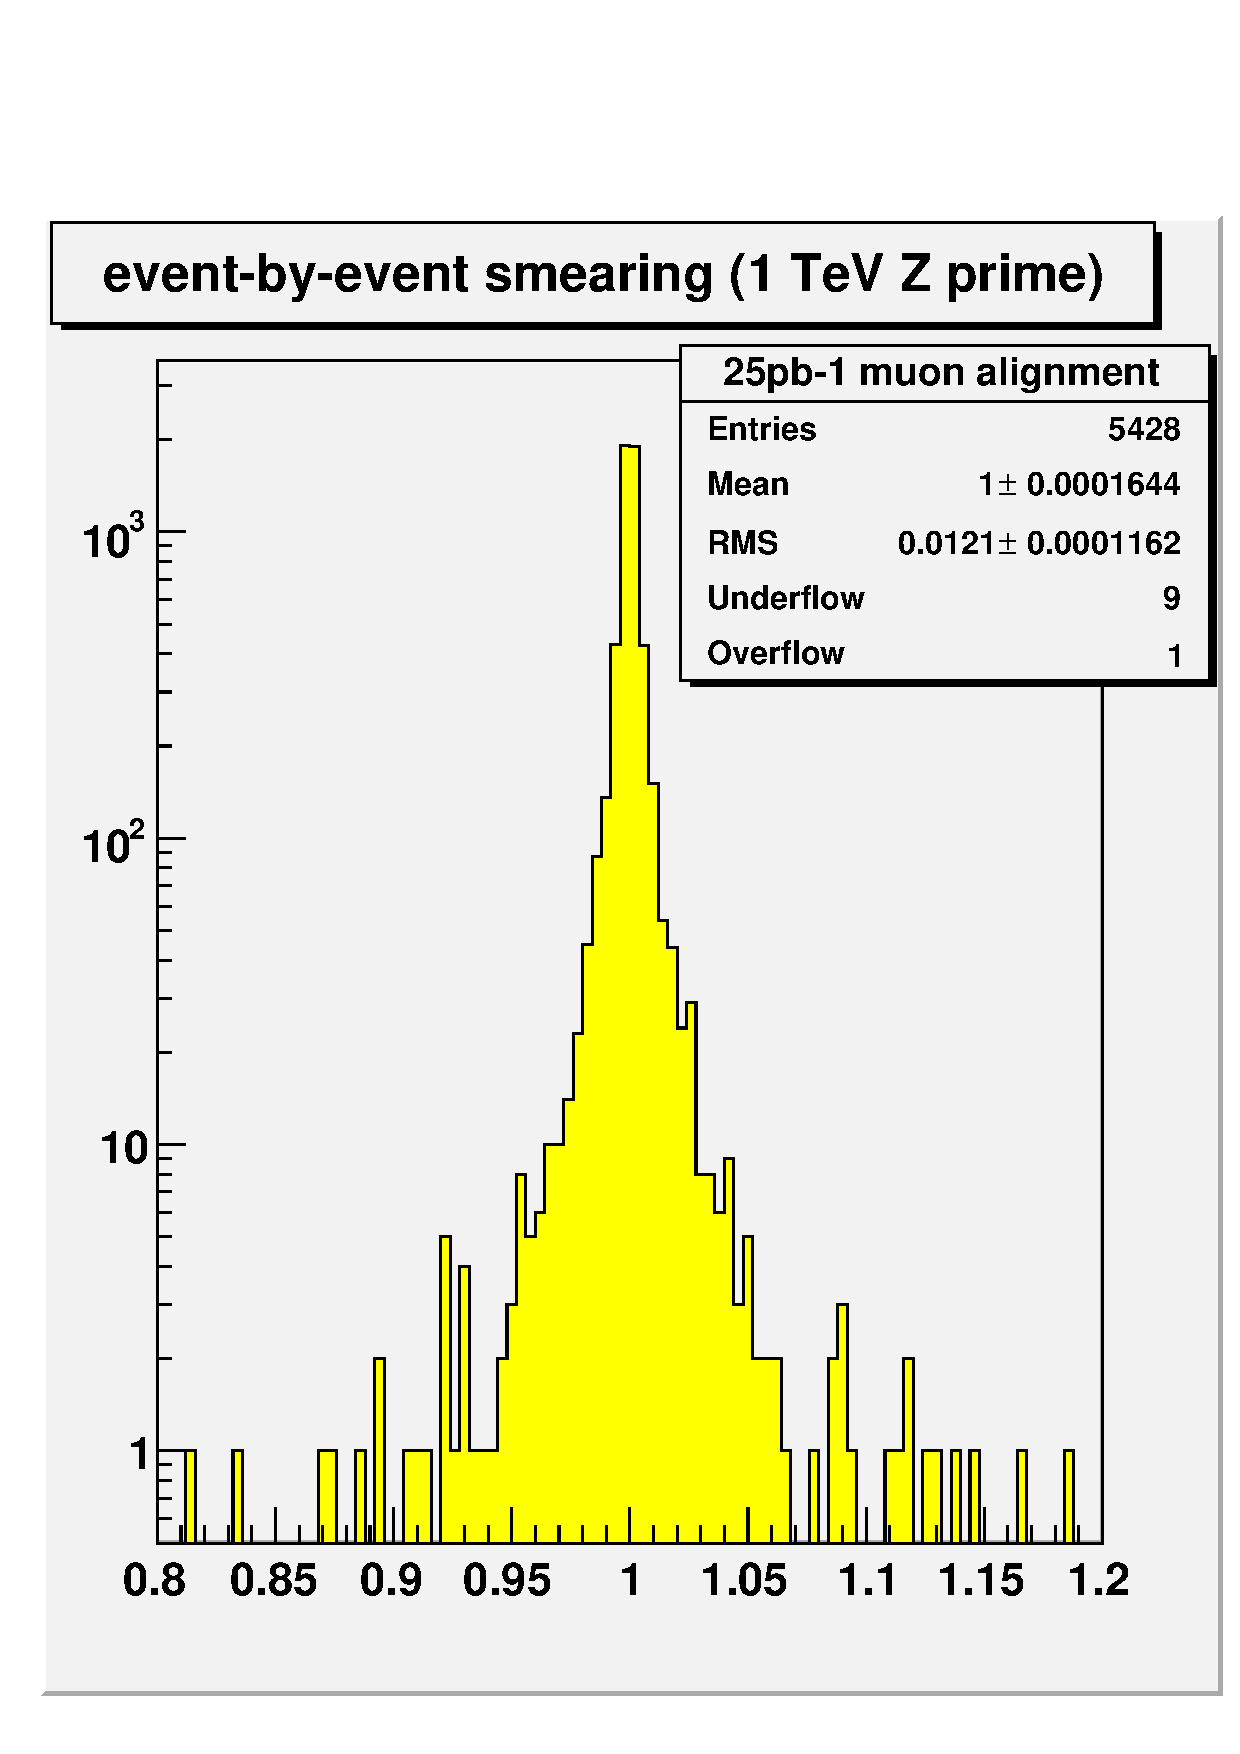
\includegraphics[width=\linewidth]{smearing_events100k.pdf}
\end{columns}
\end{frame}

\begin{frame}
\frametitle{Helps to express effect more quantitatively}

RMS of event-by-event $\displaystyle \frac{\mbox{misaligned di-muon mass}}{\mbox{ideal di-muon mass}}$

\vspace{0.75 cm}
\renewcommand{\arraystretch}{1.2}
\begin{tabular}{c c c c c}
Source of alignment & $Z'$(1000) & $Z'$(2000) & DY(1000) & DY(2000) \\\hline
1k $\mu$ (0.25~pb$^{-1}$) & 6.0\% & 5.5\% & 4.8\% & 6.6\% \\
10k $\mu$ (2.5~pb$^{-1}$) & 1.8\% & 1.7\% & 1.6\% & 2.1\% \\
100k $\mu$ (25~pb$^{-1}$) & 1.2\% & 1.1\% & 1.0\% & 1.3\% \\
325k $\mu$ (82~pb$^{-1}$) & 1.0\% & 1.0\% & 0.7\% & 1.2\% \\\hline
high $|\vec{p}|$ ($>$ 60~GeV) & 1.0\% & 1.0\% & 0.8\% & 1.2\% \\
low $|\vec{p}|$ (20--60~GeV) & 1.7\% & 1.7\% & 1.5\% & 2.1\%
\end{tabular}

\vspace{0.5 cm}
``Restricting to high $|\vec{p}|$ is like getting a factor of ten more tracks''
\end{frame}

\begin{frame}
\frametitle{Not shown at EMU: effect of tracker misalign at high $\eta$}
\begin{columns}
\column{0.7\linewidth}
\mbox{ } \hfill Outer endcap \hfill \hfill Inner endcap \hfill \mbox{ }

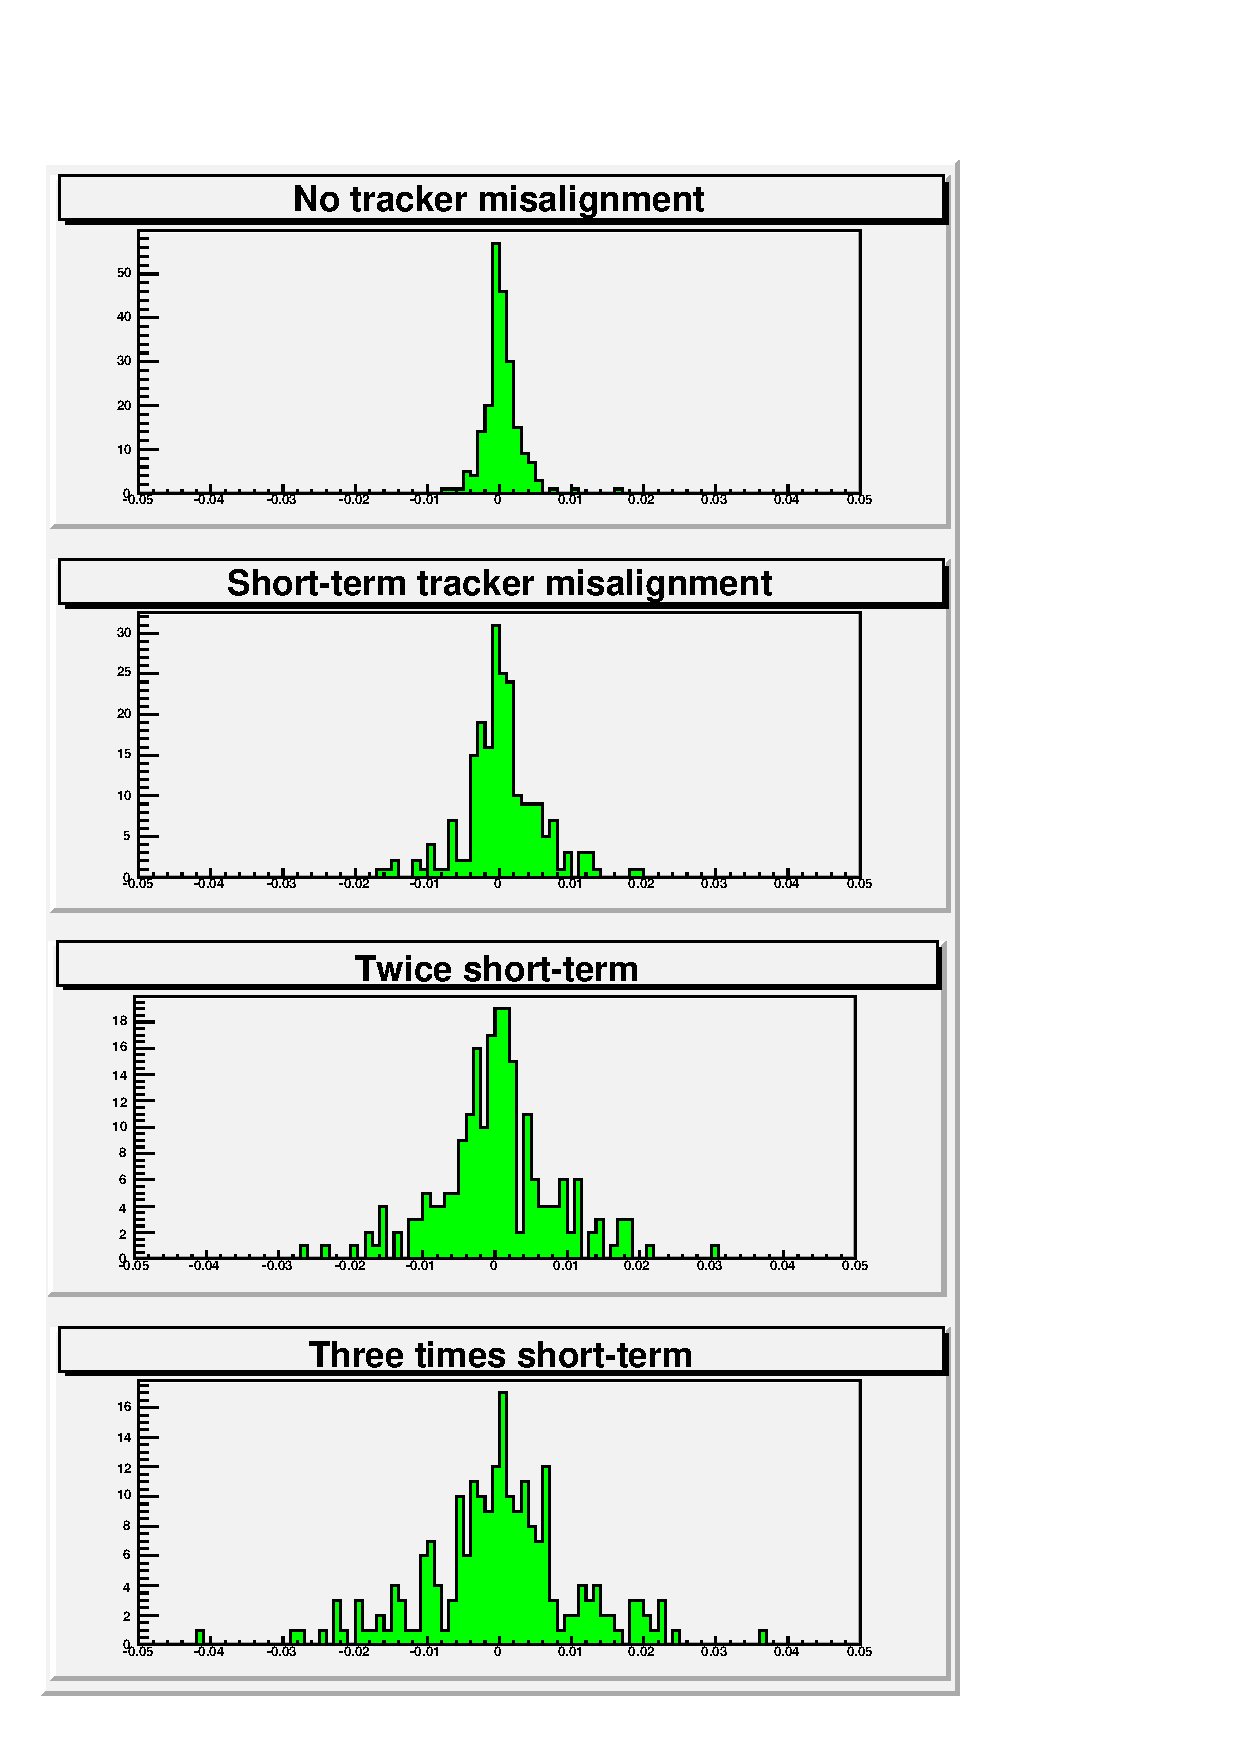
\includegraphics[width=0.5\linewidth]{trackerdep_outer_endcap.pdf}
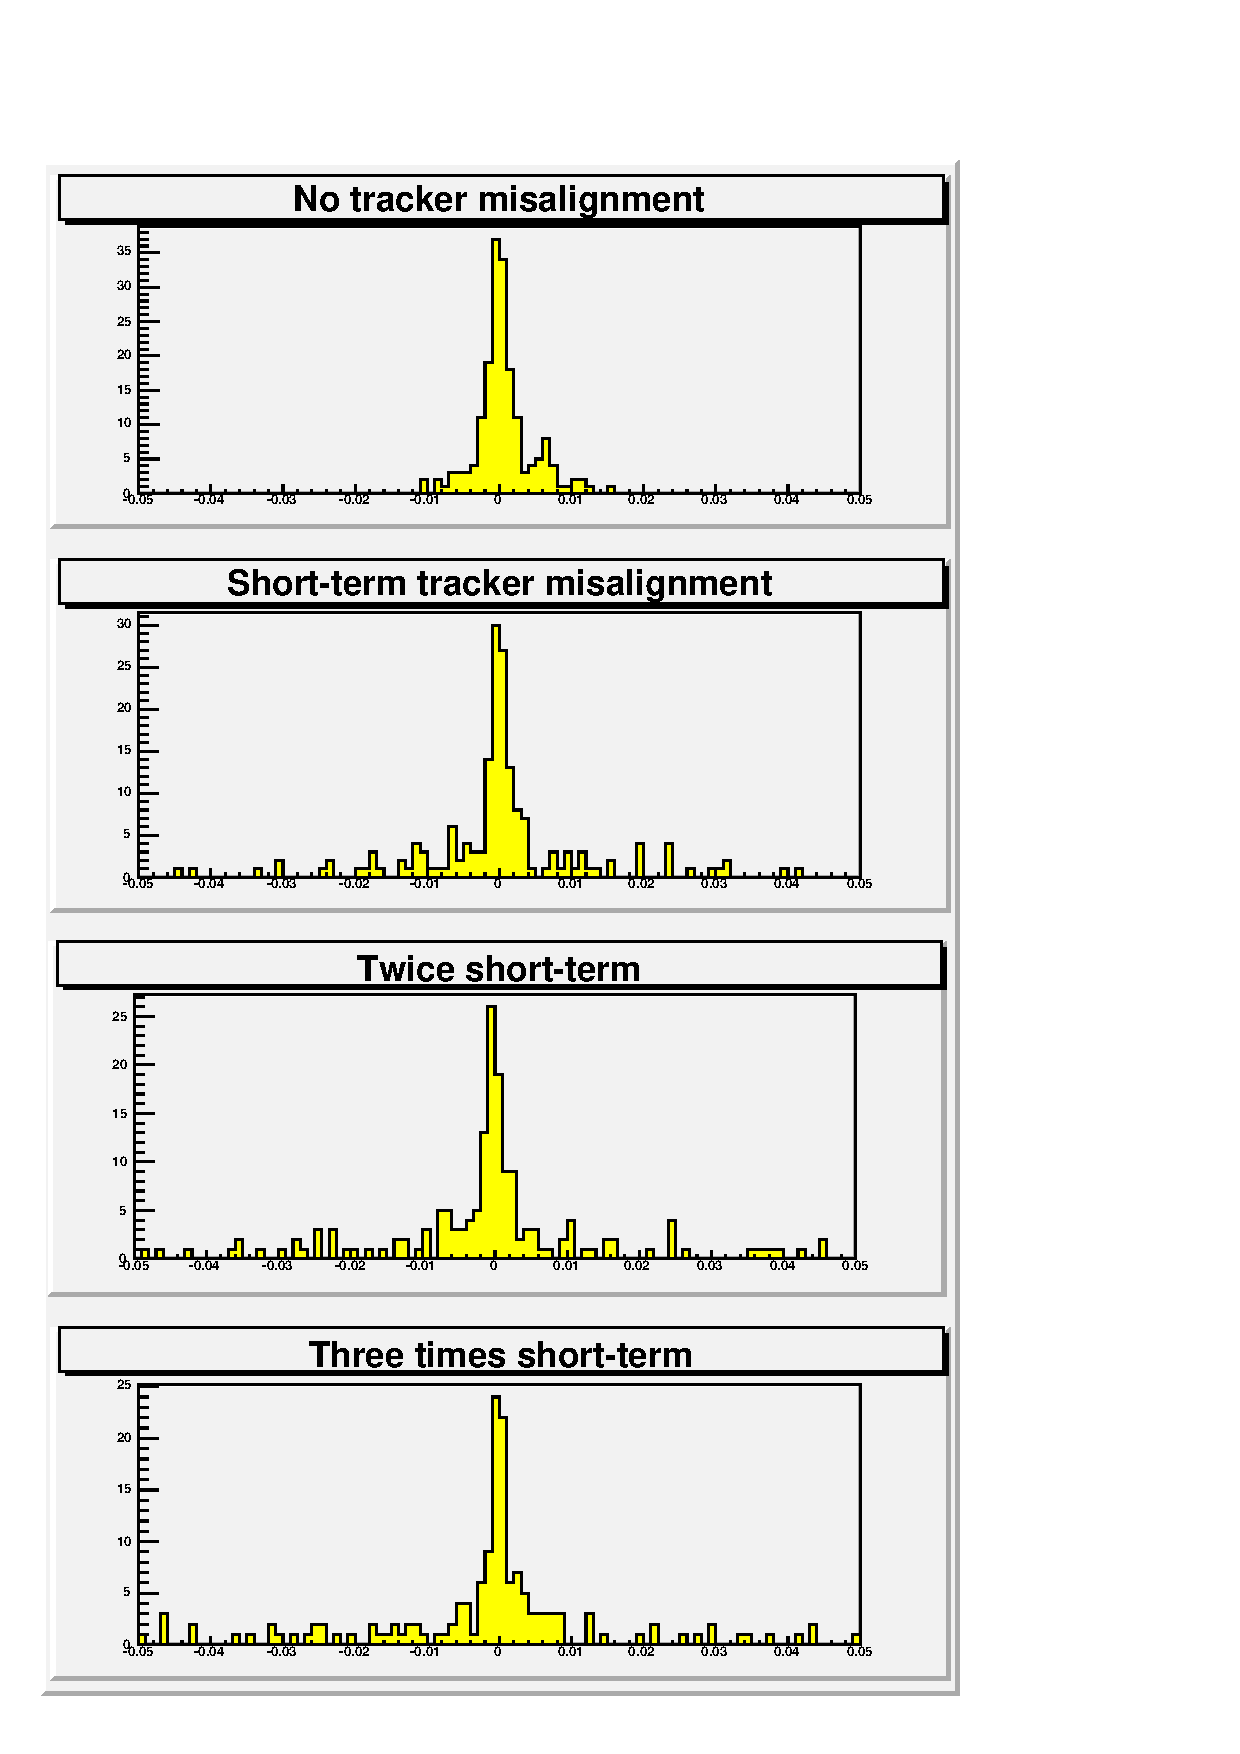
\includegraphics[width=0.5\linewidth]{trackerdep_inner_endcap.pdf}
\column{0.36\linewidth}

\mbox{\hspace{-0.5 cm}} 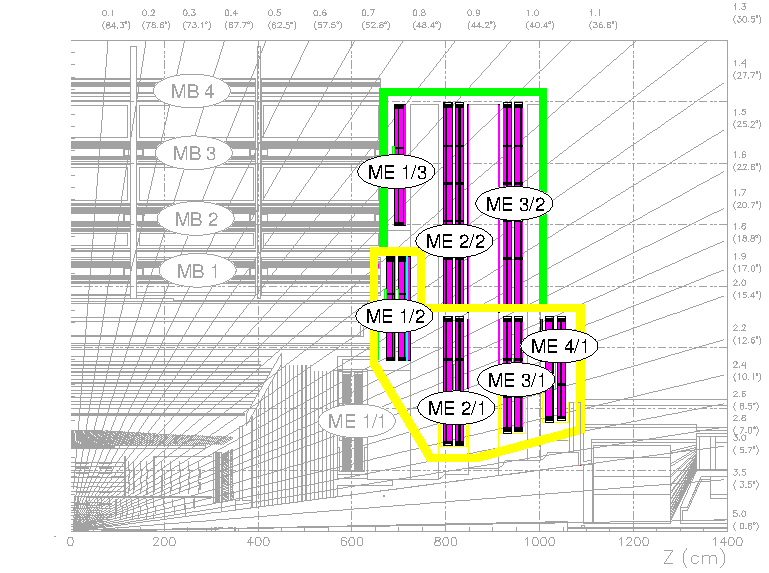
\includegraphics[width=\linewidth]{outer_inner_endcap.pdf}

\vspace{0.2 cm}
Outer endcap (1/3, 2/2, 3/2) only widens

\vspace{0.2 cm}
But inner endcap (1/2, $N$/1) gets more outliers

\vspace{0.2 cm}
May need to apply standalone procedure to these, if tracker is bad

\end{columns}
\end{frame}

\begin{frame}
\frametitle{Tracker systematic}

\vspace{-1.3 cm}
\mbox{ }\hfill
\begin{minipage}{0.5\linewidth}
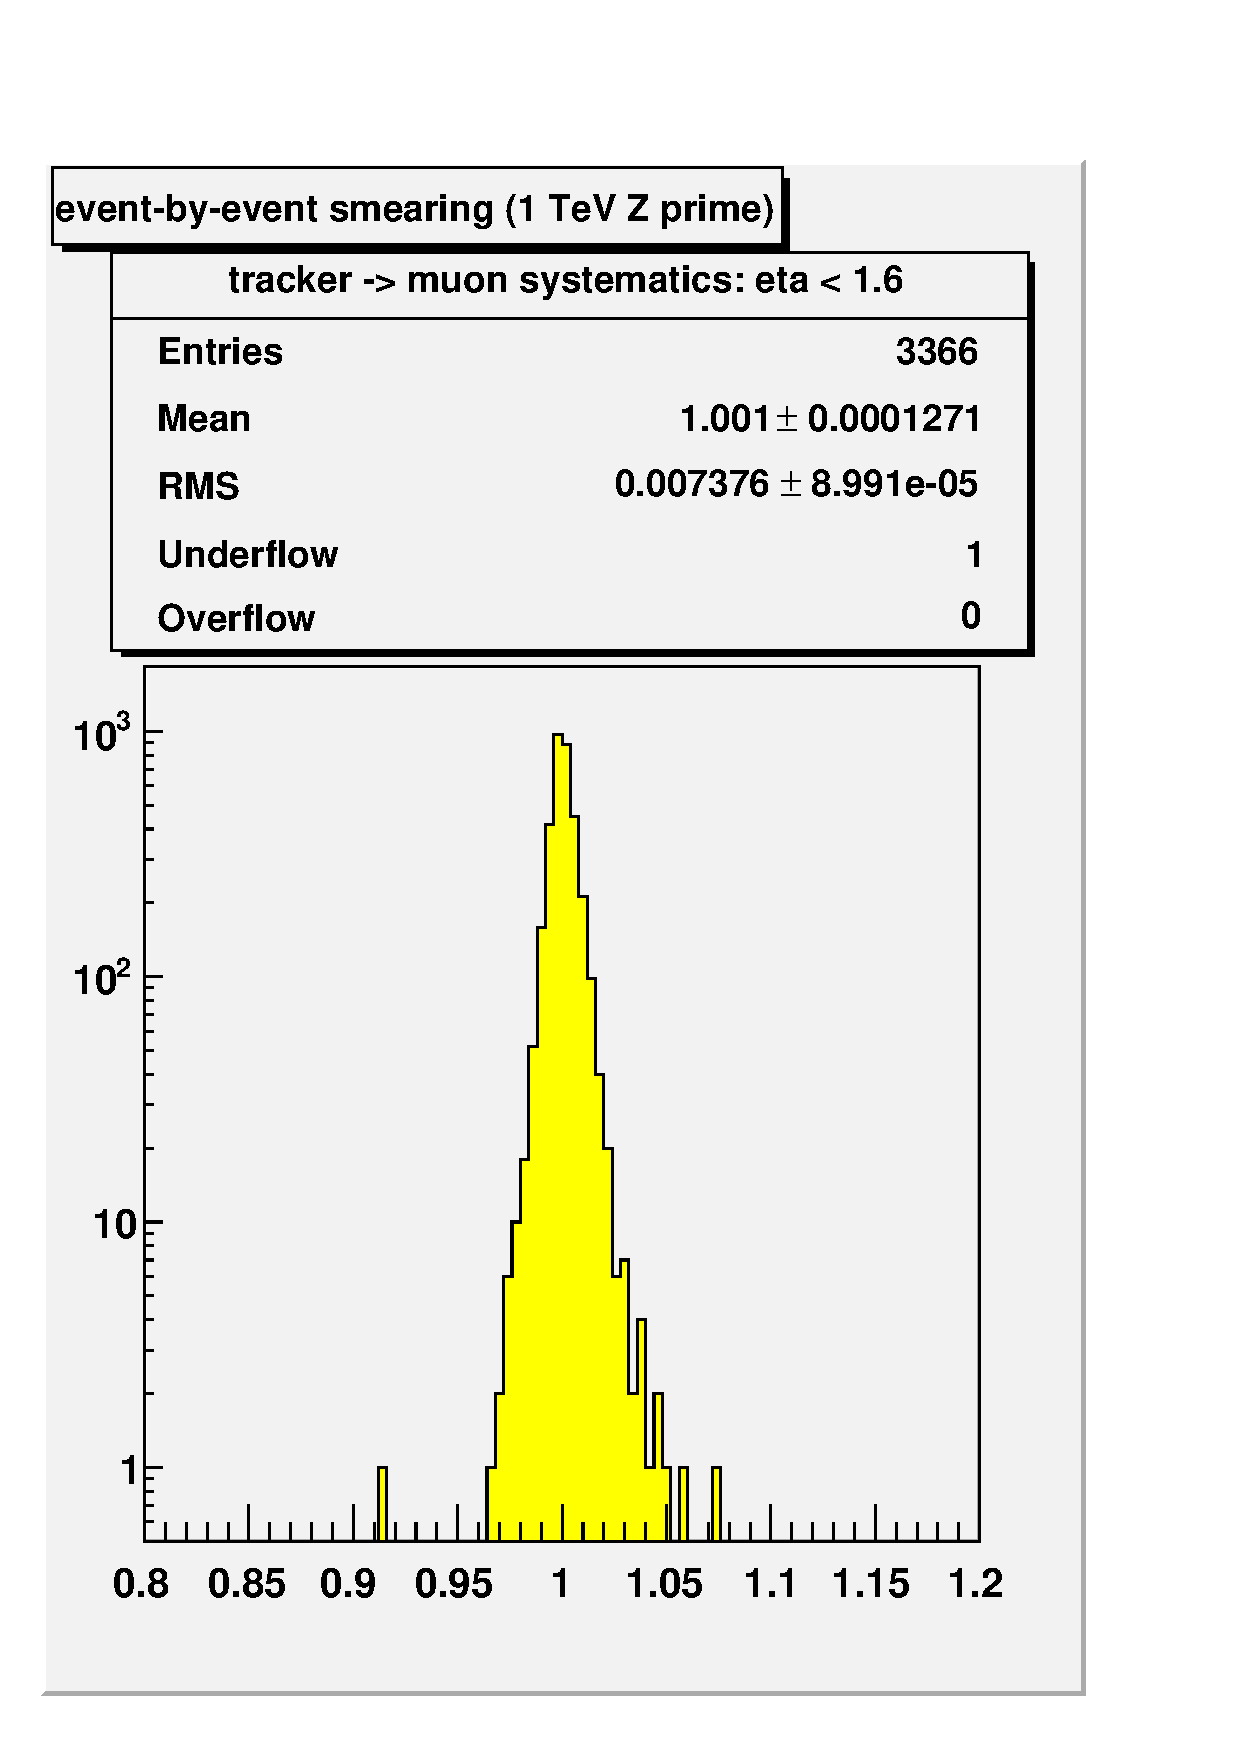
\includegraphics[width=0.5\linewidth]{tracker_systematics_low_eta.pdf}
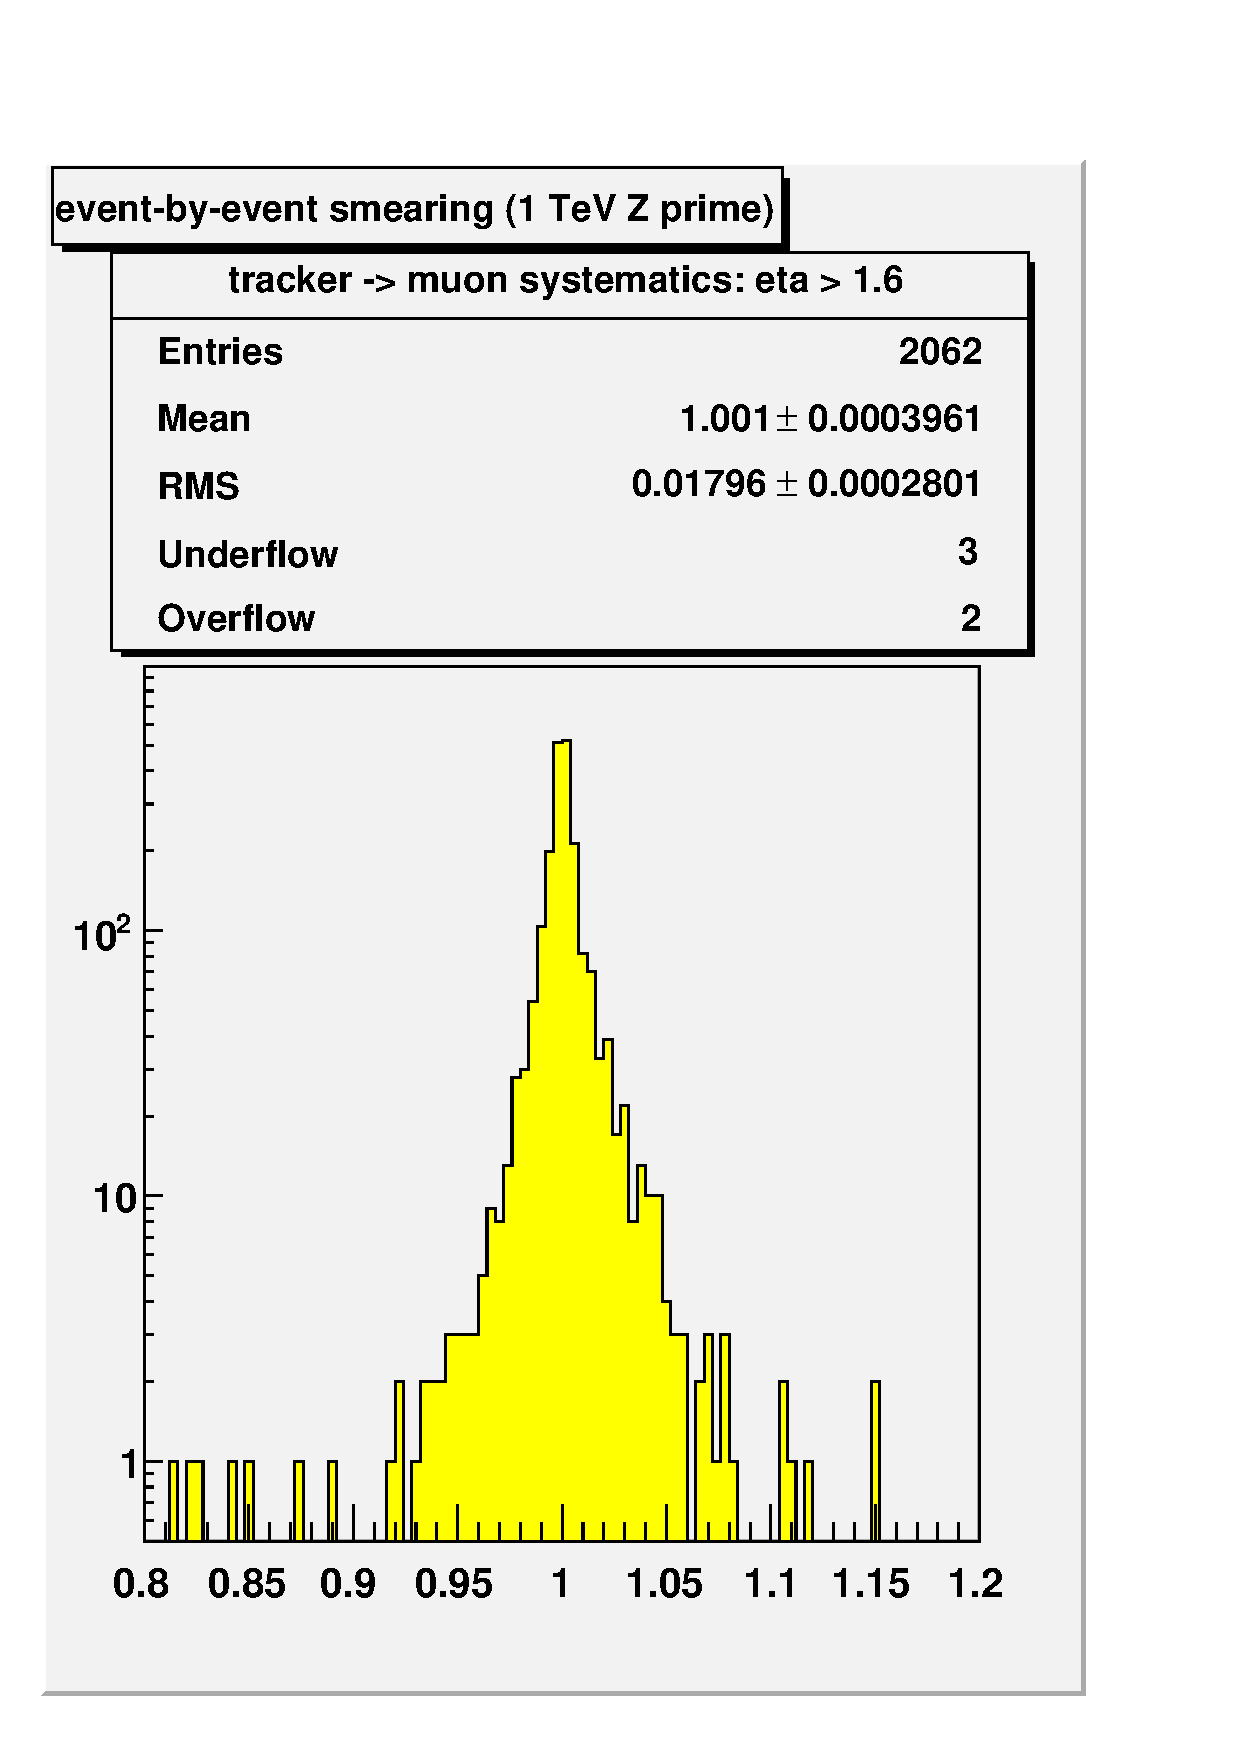
\includegraphics[width=0.5\linewidth]{tracker_systematics_high_eta.pdf}
\end{minipage}

\vspace{0.5 cm}
RMS of $\displaystyle \frac{\mbox{tracker and muon misaligned di-muon mass}}{\mbox{tracker misaligned di-muon mass}}$

\vspace{0.5 cm}
\renewcommand{\arraystretch}{1.2}
\begin{tabular}{c c c c c}
 & $Z'$(1000) & $Z'$(2000) & DY(1000) & DY(2000) \\\hline
Both $\mu$'s in $|\eta| < 1.6$ & 0.7\% & 0.9\% & 0.5\% & 1.0\% \\
One in $|\eta| > 1.6$ & 1.8\% & 1.5\% & 1.3\% & 2.0\% \\
\end{tabular}
\end{frame}

\begin{frame}
\frametitle{Conclusions}
\begin{itemize}\setlength{\itemsep}{0.1cm}
\item In even the worst sample alignments, the tails in the accuracy
distribution (outlier chambers) are not large enough to significantly
smear the Drell-Yan distribution.  (As a background to high-mass
resonances, they are only increased by tens of percent by alignment.)

\item The second moment of the distribution (RMS) matters most: $Z'$
peaks are deflated by about a factor of 2.

\item Careful!  I'm comparing muon alignment output (realistic) with
tracker alignment scenario (possibly pessimistic).

\item Standalone muon analysis would be cleaner, but less relevant to
physics goals

\item Perhaps I should look at a less digested distribution:
event-by-event smearing of individual tracks as a function of
momentum.  I'd still have to detangle tracker misalignment effects
from muon misalignment effects.
\end{itemize}
\label{numpages}
\end{frame}

\end{document}
